% ============= Package Einstellungen & Sonstiges ============= 
\documentclass[a4paper,12pt]{report}
\usepackage[left= 2.5 cm,right = 2.5 cm, bottom = 2.5 cm]{geometry}
\usepackage[onehalfspacing]{setspace}

\usepackage[
pdftitle={Studienarbeit},
pdfsubject={Entwicklung einer smarten Bewässerungslösung mit Web-Anbindung},
pdfauthor={Maximilian Schüller, Fynn Thierling, Justus Siegert, Lukas Maier, Timon Kleinknecht},
pdfkeywords={},	
hidelinks %Links nicht einrahmen
]{hyperref}

\usepackage[utf8]{inputenc}
\usepackage[ngerman]{babel}
\usepackage[T1]{fontenc}

\usepackage{fancyhdr}
\usepackage{color}
\usepackage{csquotes}
%\usepackage{cite}
\usepackage[backend=biber, autocite=inline, style=ieee, natbib=true]{biblatex}
\addbibresource{literatur.bib}
\DefineBibliographyStrings{ngerman}{andothers = {{et\,al\adddot}},}
\usepackage{url}

\usepackage{graphicx} %für Einbindung von Grafiken
\graphicspath{{img/}} %Pfad für Grafiken
\usepackage{svg}
\usepackage{amsmath}

\usepackage{pdfpages}

\usepackage{todonotes}

%\usepackage[printonlyused]{acronym}
% Akronymverzeichnis
\usepackage{hyperref}
\usepackage{array}
\usepackage{supertabular}
\usepackage{acro}
\acsetup{make-links}
%Überschrift "Abkürzungsverzeichnis" setzen
\section*{Abkürzungsverzeichnis}
\addcontentsline{toc}{section}{Abkürzungsverzeichnis}
\begin{acronym}[STRIDE]
	%\acro{EXP}{example}	-> Im text verwenden mit \ac{EXP}	
	
\end{acronym}

\usepackage{minted} %für Darstellung von Code
\usepackage{float}
\usepackage[german]{varioref} %für schönere Referenzierung von Abbildungen

\fancyhead[L]{} % Linke Kopfzeile leer lassen

\usepackage{xspace}

% Define a command to ensure consistent space after acronym
%\newcommand{\acspace}{\xspace\hspace{1em}}

\makeatletter
\renewcommand*{\aclabelfont}[1]{\textbf{\acsfont{#1}\acspace}}
\makeatother


\newcommand{\source}[1]{\vspace{1ex}\noindent{\small \textit{Quelle: #1}}}

\newcommand{\initializeBibliography}{
	\ihead{}
	\printbibliography[title=\Literaturverzeichnis] 
	\cleardoublepage
}

\usepackage{enumitem}
\usepackage{amssymb}

\usepackage{listings}
\usepackage{listings-golang}
\usepackage{xcolor}  % Optional, für zusätzliche Farbanpassungen
\lstset{ 
	language=Python,                % Programmiersprache
	basicstyle=\ttfamily\scriptsize,     % Grundschriftart (monospace) und -größe
	keywordstyle=\bfseries\color{blue}, % Schlüsselwörter fett und blau
	commentstyle=\itshape\color{green!50!black}, % Kommentare kursiv und grün
	stringstyle=\color{red},        % Strings rot
	numbers=left,                   % Zeilennummern links anzeigen
	numberstyle=\tiny\color{black},  % Stil der Zeilennummern (klein und grau)
	stepnumber=1,                   % Jede Zeile nummerieren
	numbersep=8pt,                  % Abstand der Zeilennummern zum Code
	backgroundcolor=\color{gray!10},  % Hintergrundfarbe des Codes (weiß)
	frame=single,                   % Rahmen um den Code
	rulecolor=\color{black},        % Rahmenfarbe
	captionpos=b,                   % Position des Titels (unten)
	breaklines=true,                % Zeilen umbrechen, wenn sie zu lang sind
	breakatwhitespace=true,         % Zeilenumbrüche nur an Leerzeichen
	showstringspaces=false,         % Leerzeichen in Strings nicht anzeigen
	tabsize=4,                      % Breite eines Tabs
	%escapeinside={(*@}{@*)},        % LaTeX-Befehle innerhalb des Codes
	morekeywords={print,def,class}, % Zusätzliche Schlüsselwörter für Python
	extendedchars=true,             % Unterstützt erweiterte Zeichen (z. B. Umlaute)
}
% Label für Listings ändern
\renewcommand{\lstlistingname}{Beispiel}
\newcommand{\code}[1]{\colorbox{gray!20}{\consola #1}}

\usepackage{titlesec}
\titleformat{\chapter}[hang]
  {\normalfont\huge\bfseries}
  {\thechapter\quad}
  {0pt}
  {} 


% ============= Dokumentbeginn =============
\begin{document}
	
	%Titelseite
	\thispagestyle{empty}
\begin{center}
\begin{tabular}{p{\textwidth}}
		
\begin{center}
	\textbf{\Large{\textsc{
			Entwicklung einer smarten Bewässerungslösung mit Web-Anbindung
	}}}
\end{center}

\vspace{1em}
\vspace{1em}
\vspace{1em}

\begin{center}
	\Large{Studienarbeit}
\end{center}

\vspace{1em}

\begin{center}
	im Rahmen des \\
	\large{\textbf{Bachelor of Science (B.Sc.)}} 
\end{center}

\vspace{1em}

\begin{center}
	des Studiengangs Informatik Cyber Security \\
	der Dualen Hochschule Baden-Württemberg Mannheim
\end{center}

\vspace{1em}
\vspace{1em}

\begin{center}
	vorgelegt von
\end{center}

\begin{center}
	\textbf{Maximilian Schüller, Fynn Thierling, Justus Siegert,\\Lukas Maier, Timon Kleinknecht}
\end{center}

\vspace{1em}
\vspace{1em}

\begin{center}
	\today
\end{center}
\end{tabular}
\end{center}
	
	\cleardoublepage
	\pagenumbering{roman}
	
	%------------- Erklärung der Eigenleistung-----------

	\pagebreak
\hspace{0pt}
\vfill
\begin{center}
    \large{Erklärung der Eigenleistung}
\end{center}
\vspace{1em}
\begin{center}
    \textit{Hiermit erklären wir, dass wir die vorliegende Studienarbeit selbstständig und ohne fremde Hilfe verfasst haben. Wir haben keine anderen als die angegebenen Quellen und Hilfsmittel benutzt. Darüber hinaus erklären wir, dass im Rahmen des Schreibprozesses KI-gestützte Werkzeuge (ChatGPT) zur Umformulierung von Textstellen verwendet wurden. Wir bestätigen hiermit, dass alle verwendeten Quellenangaben korrekt sind und die inhaltliche Verantwortung für die Arbeit uneingeschränkt bei uns liegt.}
\end{center}

\begin{tabular}{>{\centering\arraybackslash}p{0.5\textwidth} >{\centering\arraybackslash}p{0.5\textwidth}}
  \includegraphics[height=2\baselineskip, keepaspectratio]{img/MS_Unterschrift.png}
  &
  \includegraphics[height=2\baselineskip, keepaspectratio]{img/FT_Unterschrift.png}
  \\
  Maximilian Schüller & Fynn Thierling \\
  \includegraphics[height=2\baselineskip, keepaspectratio]{img/JS_Unterschrift.png}
  &
  \includegraphics[height=2\baselineskip, keepaspectratio]{img/LM_Unterschrift.jpg}
  \\
  Justus Siegert & Lukas Maier \\
  \includegraphics[height=2\baselineskip, keepaspectratio]{img/Unterschrift_TK.jpg}
  &
  \\
  Timon Kleinknecht & Mannheim, 15.04.2025
\end{tabular}


\vfill
\hspace{0pt}
\pagebreak

	\newpage

	%------------- Abstract -------------
	% Abstract in English
\section*{Abstract}
\addcontentsline{toc}{section}{Abstract}

\newpage

% Abstract in Deutsch
\section*{Abstrakt}
\addcontentsline{toc}{section}{Abstrakt}


	\newpage
	
	%------------- Inhaltsverzeichnis -------------
	\tableofcontents
	
	%------------- Abkürzungsverzeichnis -------------
	%%Überschrift "Abkürzungsverzeichnis" setzen
\section*{Abkürzungsverzeichnis}
\addcontentsline{toc}{section}{Abkürzungsverzeichnis}
\begin{acronym}[STRIDE]
	%\acro{EXP}{example}	-> Im text verwenden mit \ac{EXP}	
	
\end{acronym}
	\printacronyms[template=supertabular]
    \addcontentsline{toc}{chapter}{Abkürzungen}
    \newpage
	
	%------------- Abbildungsverzeichnis -------------
	\section*{Abbildungsverzeichnis}
	\addcontentsline{toc}{section}{Abbildungsverzeichnis}
	\renewcommand{\listfigurename}{} % Verhindert doppelten großen Titel
	\newpage

	
	%------------- Tabellenverzeichnis -------------
	\section*{\listtablename}
	\addcontentsline{toc}{section}{\listtablename}
	\renewcommand{\listtablename}{} % Verhindert doppelten großen Titel
	\newpage

	
	% pagestyle für restliches Dokument aktivieren
	\pagestyle{fancy}
	\pagenumbering{arabic}
	


	%------------- Einleitung -------------
	\chapter{Einleitung}
	\section{Motivation}
\label{sec:Motivation}

Pflanzen gehören in Deutschland und Europa fest zum Alltag in Wohnung und Garten. Laut einer repräsentativen Umfrage aus dem Jahr 2020 besitzen rund drei Viertel der Bundesbürger:innen (74\,\%) Zimmerpflanzen in ihrem Zuhause; auch auf Balkonen (35\,\%), Terrassen (30\,\%) und Fensterbänken (21\,\%) grünt es, während nur etwa 10\,\% ganz ohne Pflanzen leben\autocite{pflanzenbesitz_de}. Dieses „grüne Zuhause“ liegt im Trend und gewann insbesondere während der COVID-19-Pandemie an Bedeutung – viele Menschen entdeckten 2020 im Home-Office ihre Liebe zu Haus- und Gartenpflanzen neu\autocite{pflanzenbesitz_de}. Entsprechend stieg der Absatz: Der deutsche Markt für Blumen und Zierpflanzen erreichte nach Jahren der Stagnation 2020 ein Rekordvolumen von 9{,}4\,Mrd.\,€\autocite{stihl_gartenbarometer}. Ähnlich hohe Werte zeigen sich europaweit, wo Pflanzen als wichtiger Teil der Wohn- und Lebensqualität gelten. Neben dekorativen Aspekten werden Zimmer- und Gartenpflanzen aufgrund positiver Effekte wie besserer Luftqualität und Stressreduktion geschätzt\autocite{pflanzenbesitz_de}. Die hohe Verbreitung und Wertschätzung von Pflanzen in Privathaushalten bildet den Ausgangspunkt für die Betrachtung, wie ihre Pflege im Alltag unterstützt werden kann.

Allerdings stehen viele Pflanzenbesitzer:innen vor praktischen Herausforderungen bei der Pflege ihres „grünen Mitbewohners“. Im hektischen Alltag wird das Gießen leicht vergessen oder unregelmäßig vorgenommen; umgekehrt gießen unerfahrene Halter oft zu viel aus Sorge um die Pflanze. Studien bestätigen, dass Überwässerung der häufigste Grund für das Eingehen von Zimmerpflanzen ist\autocite{pflanzenpflege_fehler}. Generell erfordert jede Pflanzenart spezifische Kenntnisse zu Wasser- und Nährstoffbedarf, Lichtverhältnissen etc., über die im privaten Umfeld nicht immer ausreichend Wissen vorhanden ist. So gaben in einer Umfrage lediglich 37\,\% der befragten Frauen und 20\,\% der Männer an, einen „grünen Daumen“ zu haben\autocite{pflanzenbesitz_de} – die Mehrheit traut sich die optimale Pflanzenpflege also eher nicht zu. Hinzu kommt, dass während Urlaubs- oder Abwesenheitszeiten oft keine Betreuung für die heimischen Gewächse sichergestellt ist. Tatsächlich vermissten in einer Befragung 26\,\% der Pflanzenhalter:innen ihre Zimmerpflanzen im Urlaub sogar mehr als die Kolleg:innen\autocite{pflanzenbesitz_de}, was die emotionale Bindung und zugleich das Problem der Versorgung in dieser Zeit verdeutlicht. Diese Pflegeherausforderungen führen dazu, dass viele privat gehaltene Pflanzen Schäden nehmen oder vorzeitig absterben.

Die Folgen von falscher oder unregelmäßiger Pflege sind in Zahlen beträchtlich. Hochrechnungen zufolge überlebt ein erheblicher Teil der gekauften Zierpflanzen nicht lange: Etwa 40\,\% der Pflanzen gehen bereits in der Lieferkette zugrunde, und weitere rund 35\,\% sterben später in den Wohnungen der Kundschaft\autocite{pflanzensterben_statistik}. Mit anderen Worten wird fast die Hälfte aller gekauften Haus- und Gartenpflanzen letztlich aufgrund suboptimaler Bedingungen oder Pflegefehler nicht dauerhaft erhalten. Auch Verbraucherumfragen deuten auf dieses Problem hin. Beispielsweise gab über ein Drittel der Hobbygärtner in einer aktuellen Erhebung an, jedes Jahr ein bis zwei Zimmerpflanzen zu verlieren\autocite{pflanzensterben_statistik}. Solche Verluste sind nicht nur emotional enttäuschend für Pflanzenliebhaber, sondern bedeuten auch Ressourcenverschwendung – insbesondere von Wasser, Zeit und Geld. Schätzungen aus den USA zeigen etwa, dass jüngere „Plant Parents“ im Durchschnitt schon mehrere ihrer erworbenen Pflanzen unbeabsichtigt zum Eingehen gebracht haben. Diese Zahlen unterstreichen die Notwendigkeit, neue Wege zu finden, um häufige Pflegefehler zu vermeiden und die Lebensdauer der Pflanzen zu verlängern.

Technologische Lösungen im Sinne von \textit{Smart Gardening} setzen hier an und versprechen Abhilfe. Insbesondere automatische Bewässerungssysteme für den Heimgebrauch bieten die Möglichkeit, den Gießvorgang zu optimieren und zu automatisieren. Solche Systeme kombinieren oft Sensoren (etwa für Bodenfeuchte oder Licht) mit internetfähigen Steuerungen, um den Pflanzen exakt bei Bedarf und in der richtigen Menge Wasser zuzuführen. Erste Ansätze sind bereits auf dem Markt verfügbar – von App-gesteuerten Bewässerungscomputern bis hin zu smarten Pflanzentöpfen mit Selbstbewässerungs-Funktion. Die Akzeptanz solcher \textit{Smart-Home}-Technologien im Garten- und Pflanzenbereich steigt kontinuierlich. Laut dem STIHL-Gartenbarometer 2022 nutzen bereits rund 7\,\% der deutschen Gartenbesitzer smarte Garden-Lösungen, und etwa 30\,\% wünschen sich zukünftig solche automatisierten Helfer\autocite{stihl_gartenbarometer}. Dabei stehen Bewässerungsautomationen an erster Stelle der Wunschliste: 83\,\% der Befragten mit Smart-Gardening-Interesse nennen ein automatisches Bewässerungssystem als besonders gefragte Lösung. Diese Nachfrage spiegelt sich auch in anderen Ländern wider. Beispielsweise glauben in Österreich über 60\,\% der Gartenbesitzer, dass sich der Wasserverbrauch durch automatisierte Bewässerungsanlagen deutlich optimieren lässt. Moderne Systeme können Wetterdaten oder Bodensensoren einbeziehen, um nur dann zu wässern, wenn die Pflanze es wirklich benötigt – eine Technik, die den Pflanzenstress reduziert und zugleich Wasserverschwendung vorbeugt. Aktuelle Untersuchungen zeigen denn auch, dass intelligente Bewässerungssteuerungen den Wasserverbrauch im Garten gegenüber herkömmlichen Timern erheblich senken können (um etwa 20–40\,\% je nach System).

Mehrere übergeordnete Trends begünstigen die Verbreitung von smarten Pflanzenpflege-Systemen. Zum einen führt die Urbanisierung dazu, dass immer mehr Menschen auf kleinem Raum in Städten leben – in Deutschland etwa 78\,\% der Bevölkerung\autocite{urbanisierung_de} – und sich dennoch nach Natur im eigenen Umfeld sehnen. Insbesondere Stadtbewohner ohne Garten kultivieren vermehrt Zimmerpflanzen oder Balkongrün, sind aber beruflich oft stark eingebunden. Eine automatische Bewässerung kann hier den Pflegeaufwand mindern und sicherstellen, dass Pflanzen trotz hektischem Alltag oder Abwesenheiten ausreichend versorgt werden. Zum anderen rückt Nachhaltigkeit in den Fokus: Wassermanagement und effiziente Ressourcennutzung gewinnen an Bedeutung, da die Auswirkungen des Klimawandels – etwa häufigere Sommerdürreperioden – auch private Gärten und Balkone betreffen. In Umfragen äußern fast zwei Drittel der Befragten die Erwartung, dass digitale Technologien im Garten helfen können, den Klimawandel abzuschwächen, und nennen den schonenden Umgang mit Wasser als oberste Priorität. Smart-Bewässerungssysteme erfüllen genau diesen Zweck, indem sie bedarfsgerecht gießen und Überwässerung verhindern. Schließlich trägt auch die allgemeine Verbreitung von \textit{Internet of Things}-Anwendungen im Haushalt dazu bei, dass vernetzte Lösungen immer selbstverständlicher werden. Der europäische Smart-Home-Markt verzeichnet hohe Wachstumsraten und wird 2024 bereits auf über 22\,Mrd.\,US-\$ geschätzt\autocite{iot_trend}. Vernetzte, per App oder Sprache steuerbare Geräte – vom Thermostat bis zur Lichtsteuerung – gehören zunehmend zum Alltag. Diese Entwicklung macht auch vor dem Bereich der Pflanzenpflege nicht Halt: Die Nutzerakzeptanz für digitale Helfer im Haushalt schafft ein günstiges Umfeld für \textit{Smart Gardening}-Innovationen.

Insgesamt ist die Einführung eines smarten Bewässerungssystems im heimischen Umfeld vor dem Hintergrund dieser Fakten sowohl technisch zeitgemäß als auch gesellschaftlich sinnvoll. Die weit verbreitete Haltung von Zimmer- und Gartenpflanzen einerseits und die häufig auftretenden Pflegeprobleme andererseits schaffen ein deutliches Bedürfnis nach Unterstützung. Automatisierte Bewässerungslösungen können hier einen doppelten Nutzen stiften: Sie helfen Pflanzenbesitzer:innen, ihre grünen Schützlinge zuverlässig und fachgerecht zu versorgen, und tragen zugleich zu Nachhaltigkeit und Komfort bei. Indem ein smartes Bewässerungssystem Wasser bedarfsgerecht dosiert und den Pflegeprozess vereinfacht, steigert es die Überlebensrate und Vitalität der Pflanzen und entlastet den Menschen von Routineaufgaben. Die vorliegenden Studien, Statistiken und Trends untermauern somit die Notwendigkeit und den Nutzen eines solchen Systems, das im Folgenden technisch konzipiert und beschrieben wird.

	\newpage
	\section{Zielsetzung}
\label{sec:Zielsetzung}

Ziel dieser Studienarbeit ist die Konzeption, Entwicklung und prototypische Umsetzung eines automatisierten Systems zur Bewässerung von Zimmerpflanzen im privaten Wohnumfeld. Es soll eine lauffähige Gesamtlösung entstehen, die aus einem Mikrocontroller als zentrale Steuereinheit, einer Backend-Infrastruktur zur Datenverarbeitung und -persistierung sowie einem benutzerfreundlichen Frontend zur Visualisierung und Steuerung besteht. Die Realisierung erfolgt im Rahmen eines \textit{Proof of Concept}, der die technische Machbarkeit sowie die Integration der Systemkomponenten demonstriert.
\\
Das zu entwickelnde System erfasst über geeignete Sensorik (z.\,B. Bodenfeuchte, Temperatur, Luftfeuchtigkeit, Lichtintensität) kontinuierlich relevante Umgebungsdaten. Diese Messwerte dienen entweder als Entscheidungsgrundlage für den Nutzer, um über die Benutzeroberfläche manuell eine Bewässerung anzustoßen, oder sie werden vom Mikrocontroller automatisch verarbeitet. Im letzteren Fall wird anhand zuvor definierter Sollwerte eine autonome Steuerung der Bewässerungseinheit realisiert. Vorrangiges Ziel ist die technische Umsetzung des automatischen Betriebsmodus. Die Konzeption und Entwicklung des manuellen Modus sowie die Integration beider Steuerungsarten in das Gesamtsystem erfolgen nachrangig und abhängig von den im Projektverlauf verfügbaren Entwicklungskapazitäten.
\\
Die Bewässerungslösung ist primär für den Einsatz in Innenräumen konzipiert. Dies umfasst insbesondere Haushalte mit Zimmerpflanzen, bei denen typische Pflegeprobleme wie unregelmäßiges Gießen oder Unsicherheit bezüglich des Wasserbedarfs adressiert werden sollen.
\\
Der konkrete Funktionsumfang des Systems wird im Verlauf des Projekts iterativ entwickelt. Eine detaillierte Beschreibung der funktionalen und nicht-funktionalen Anforderungen sowie der Zielsystemeigenschaften erfolgt in Kapitel~\ref{chap:Anforderungen}. Dabei wird angestrebt, etablierte \textit{Best Practices} der Software- und Systementwicklung zu berücksichtigen und – wo sinnvoll und realisierbar – aktuelle Technologien gemäß dem Stand der Technik (\textit{State of the Art}) zu verwenden. Gleichzeitig wird die technische Umsetzung unter Berücksichtigung der konzeptionellen Natur als \textit{Proof of Concept} gewichtet, sodass pragmatische Abwägungen hinsichtlich Komplexität, Aufwand und Ressourcen erfolgen.
\\
Insgesamt dient die Arbeit dem Ziel, ein funktional überzeugendes Demonstrationssystem zu realisieren, das eine fundierte Grundlage für weiterführende Entwicklungen, Evaluationen oder mögliche Produktivsetzungen bietet.

	\newpage
	\section{Ziel der Arbeit}
\label{sec:Ziel der Arbeit}


	\newpage
	
	% ------------- Hauptteil -------------

	\chapter{Theoretische Grundlagen}
	\section{Scrum und das Agile Manifest}
Scrum basiert auf den Grundsätzen des Agilen Manifests. Das Agile Manifest ist eine Sammlung von Priorisierungsprinzipien, die im Jahr 2001 von 17 Experten und Vertretern unterschiedlicher agiler Vorgehensweisen in Snowbird, USA, entwickelt wurde. Diese Gruppe, oft als die \glqq Snowbird 17\grqq{} bezeichnet, erkannte frühzeitig die Notwendigkeit einer neuen Ära der Softwareentwicklung. \cite{Drumond} Das Agile Manifest umfasst im Original nur 68 Wörter, aber aus diesem knappen Text wurden allgemeingültige Prinzipien abgeleitet, die bis heute die Grundlage für agile Methoden wie Scrum bilden.

Das Manifest lautet sinngemäß ins Deutsche übersetzt: 

\vspace{1em}
\glqq Wir erschließen bessere Wege, Software zu entwickeln, indem wir es selbst tun und anderen dabei helfen. Durch diese Tätigkeit haben wir diese Werte zu schätzen gelernt:

\noindent \textbf{Individuen und Interaktionen}
\vspace{-1em}
\begin{flushright}
mehr als Prozesse und Werkzeuge,
\end{flushright}
\vspace{-1em}
\textbf{Funktionierende Software}
\vspace{-1em}
\begin{flushright}
mehr als umfassende Dokumentation,
\end{flushright}
\vspace{-1em}
\textbf{Zusammenarbeit mit dem Kunden}
\vspace{-1em}
\begin{flushright}
mehr als Vertragsverhandlung,
\end{flushright}
\vspace{-1em}
\textbf{Reagieren auf Veränderung}
\vspace{-1em}
\begin{flushright}
mehr als das Befolgen eines Plans.
\end{flushright}

Das heißt, obwohl wir die Werte auf der rechten Seite wichtig finden, schätzen wir die Werte auf der linken Seite höher ein.\grqq{} \cite{Snowbird2001}

\subsection{Interpretation des Agilen Manifests in der Praxis}
Das Agile Manifest betont die Wichtigkeit von Praxisnähe in der agilen Entwicklung. Es reicht nicht aus, nur theoretische Konzepte zu entwickeln; vielmehr müssen praktische Erfahrungen gesammelt und in den Entwicklungsprozess eingebracht werden. Ein zentrales Prinzip ist, dass die Individuen und ihre Interaktionen im Vordergrund stehen. Dies bedeutet, dass ein Vorgehen gefunden werden muss, das eine effektive Kommunikation und Interaktion aller Beteiligten ermöglicht. Prozesse und Werkzeuge sollten an die Bedürfnisse der Menschen angepasst werden, nicht umgekehrt.

Darüber hinaus wird die Bedeutung funktionierender Software hervorgehoben. Der Fortschritt eines Projekts wird anhand der tatsächlich funktionierenden Software gemessen, nicht anhand umfangreicher Dokumentationen. Es ist entscheidend, dass die entwickelte Software in regelmäßigen Abständen gezeigt und von den Anwendern beurteilt wird. Dies stellt sicher, dass das Projekt auf dem richtigen Weg bleibt und die Anforderungen der Nutzer erfüllt.

Da Softwareentwicklung ein dynamischer Prozess ist, entstehen oft neue Herausforderungen oder Anforderungen, selbst bei sorgfältiger Planung. Daher ist es unerlässlich, flexibel auf Veränderungen zu reagieren. Der Erfolg eines Projekts wird daran gemessen, wie gut es sich an neue Gegebenheiten anpasst und ob daraus ein Lerneffekt resultiert, der das Projekt voranbringt.

Auch wenn das Manifest die Bedeutung von Prozessen, Dokumentation, Verträgen und Plänen anerkennt, stellt es klar, dass diese Aspekte im Vergleich zu den übergeordneten Prinzipien von geringerer Priorität sind. Sie haben jedoch weiterhin ihre Daseinsberechtigung und müssen in einem angemessenen Maße berücksichtigt werden. \cite{Wolf2011}

\subsection{Zusammenhang zwischen Scrum und dem Agilen Manifest}
Scrum operationalisiert die Prinzipien des Agilen Manifests in einem strukturierten Rahmenwerk. Die regelmäßigen Sprints und die damit verbundenen Meetings – wie das Sprint Planning, Daily Stand-ups, Sprint Reviews und Retrospektiven – fördern die Kommunikation und die Interaktion zwischen den Teammitgliedern und den Stakeholdern. Durch die iterative Natur von Scrum wird sichergestellt, dass funktionierende Software frühzeitig und kontinuierlich geliefert wird, wodurch die Kundenzufriedenheit gesteigert wird.

Die enge Zusammenarbeit mit dem Kunden, die in Scrum durch die Rolle des Product Owners verkörpert wird, gewährleistet, dass das Entwicklungsteam ständig auf die sich ändernden Anforderungen reagieren kann. Diese Flexibilität ist ein direkter Ausdruck des Wertes \glqq Reagieren auf Veränderung mehr als das Befolgen eines Plans\grqq, der im Agilen Manifest verankert ist.


\subsection{Anwendung von Scrum im Sensora-Projekt}
Aus den Grundsätzen des Agilen Manifests ergeben sich spezifische Herangehensweisen für das Sensora-Projekt:
\begin{description}
    \item[Zwischenergebnisse:] Es wird eine hohe Frequenz bei der Präsentation von Zwischenergebnissen angestrebt. Diese regelmäßigen Präsentationen bieten eine hervorragende Gelegenheit, um mit den Stakeholdern in den Dialog zu treten, Feedback zu sammeln und Verbesserungen zu identifizieren. Zudem fungieren diese Präsentationen als Indikatoren für den Projektfortschritt, wodurch erkennbar wird, ob das Projekt planmäßig voranschreitet oder ob Maßnahmen zur Kurskorrektur erforderlich sind.
    \item[Kommunikation:] Alle technischen Entscheidungen werden in enger Abstimmung mit allen Entwicklern getroffen. Dabei werden die Meinungen und Bedenken der beteiligten Personen berücksichtigt, um sicherzustellen, dass realistische Lösungen verfolgt werden. Durch diesen intensiven Austausch wird verhindert, dass Zeit und Ressourcen in ineffiziente oder unpraktikable Lösungen investiert werden. Gleichzeitig wird sichergestellt, dass das kollektive Wissen genutzt wird und potenzielle Probleme frühzeitig erkannt werden.
    \item[Lessons Learned:] Im Verlauf der Entwicklung entstehen neue Erkenntnisse, die zu neuen Möglichkeiten führen. Diese Lernfortschritte, sowohl auf fachlicher als auch auf technischer Ebene, werden genutzt, um das Projekt kontinuierlich weiterzuentwickeln und anzupassen. Die Fähigkeit, aus Erfahrungen zu lernen und diese in den Entwicklungsprozess einzubeziehen, ist ein zentraler Bestandteil des agilen Vorgehens.
\end{description}

Zusammengefasst projiziert Scrum die Werte und Prinzipien des Agilen Manifests auf einen praxisnahen und strukturierten Entwicklungsprozess, der es Teams ermöglicht, effizient und flexibel auf die Herausforderungen der Softwareentwicklung zu reagieren. Durch die Integration dieser Prinzipien in das Sensora-Projekt wird sichergestellt, dass das Produkt den Anforderungen gerecht wird und gleichzeitig eine hohe Qualität und Benutzerfreundlichkeit erreicht.

	
\section{REST APIs: Grundlagen und Best Practices}
\ac{rest} \ac{api} ist ein Architekturstil für verteilte Systeme, insbesondere für Webanwendungen. Er wurde erstmals im Jahr 2000 von Roy Thomas Fielding in seiner Dissertation eingeführt. \ac{rest} definiert eine Reihe von Prinzipien, die die Interaktion zwischen Clients und Servern in einem verteilten System standardisieren und vereinfachen sollen. Obwohl es keine offizielle Spezifikation wie einen \ac{rfc} oder eine ISO-Norm für \ac{rest} gibt, hat sich der Architekturansatz in der Praxis durchgesetzt und bildet die Grundlage für viele der heutigen Web-\acp{api}.

\ac{rest} basiert auf dem Prinzip, dass ein Webdienst über eine standardisierte Schnittstelle (\ac{api}) ansprechbar ist, bei der die Kommunikation zwischen Client und Server zustandslos ist. Das bedeutet, dass jede Anfrage vollständig ist und keine Informationen über den vorherigen Zustand benötigt werden. Diese Eigenschaft macht \ac{rest}-\acp{api} besonders skalierbar und flexibel.

\subsection{Warum REST?}

\ac{rest} hat sich gegenüber anderen Architekturansätzen wie \ac{soap} aus mehreren Gründen durchgesetzt. \ac{rest}-\acp{api} sind leichter zu implementieren und zu nutzen, da sie auf den bestehenden HTTP-Standards aufbauen. \ac{rest} nutzt die standardmäßigen HTTP-Verben (GET, POST, PUT, DELETE), um \ac{crud}-Operationen auf Ressourcen durchzuführen. Diese Einfachheit und die Nutzung bewährter Webstandards machen \ac{rest}-\acp{api} besonders attraktiv für Webanwendungen und mobile Apps, wo schnelle Entwicklung und hohe Performance entscheidend sind.

Ein weiterer Vorteil von \ac{rest} ist seine Flexibilität und die Möglichkeit zur Integration in eine Vielzahl von Plattformen und Programmiersprachen. Da \ac{rest}-\acp{api} auf dem HTTP-Protokoll basieren, können sie in nahezu jeder Umgebung eingesetzt werden, die HTTP unterstützt, was zu einer breiten Akzeptanz und Nutzung geführt hat.

\subsection{Grundlagen einer REST API}

Obwohl es kein formales Regelwerk für \ac{rest} gibt, haben sich in der Entwicklergemeinschaft einige Best Practices etabliert, die eine \ac{rest}-\ac{api} als gut definieren. Diese Best Practices sind weitgehend anerkannt und werden häufig in der Praxis angewendet:
\begin{description}
    \item[\ac{json} als Standardformat verwenden:] \ac{rest}-\acp{api} sollten \ac{json} als Standardformat für die Datenübertragung verwenden, da \ac{json} leichtgewichtig, gut lesbar und in den meisten Programmiersprachen nativ unterstützt wird.
    \item[Verwendung von Substantiven in Endpunktpfaden:] Endpunktpfade sollten Substantive anstelle von Verben verwenden, um die Ressource zu definieren, auf die die Operation angewendet wird. Beispielsweise sollte der Endpunkt \code{/users} anstelle von \code{/getUsers} verwendet werden.
    \item[Logische Verschachtelung von Endpunkten:] Endpunkte sollten logisch verschachtelt sein, um die Hierarchie der Daten widerzuspiegeln. Zum Beispiel könnte ein Endpunkt für die Bestellungen eines Benutzers \code{/users/{userId}/orders} lauten.
    \item[Fehlerbehandlung und Standard-HTTP-Fehlercodes:] Eine gute \ac{rest}-\ac{api} sollte standardisierte HTTP-Fehlercodes verwenden, um dem Client klare Rückmeldungen über den Status der Anfrage zu geben. Beispielsweise steht der Fehlercode 404 für \glqq Nicht gefunden \grqq{} und 500 für \glqq Interner Serverfehler \grqq.
    \item[Filtern, Sortieren und Paginierung:] \ac{rest}-\acp{api} sollten die Möglichkeit bieten, Ergebnisse zu filtern, zu sortieren und zu paginieren, um die Rückgabemenge zu steuern und die Effizienz zu erhöhen.
    \item[Sicherheitspraktiken:] \ac{rest}-\acp{api} sollten sichere Authentifizierungs- und Autorisierungsmechanismen verwenden, wie OAuth2 oder \ac{jwt}, um sicherzustellen, dass nur berechtigte Benutzer auf die Ressourcen zugreifen können.
    \item[Daten-Caching:] Um die Leistung zu verbessern, sollten \ac{rest}-\acp{api} Daten zwischenspeichern, wo es sinnvoll ist. Dies kann die Ladezeiten reduzieren und die Last auf dem Server verringern.
    \item[\ac{api}-Versionierung:] Eine gute \ac{rest}-\ac{api} sollte versioniert werden, um Änderungen und Verbesserungen an der \ac{api} zu ermöglichen, ohne bestehende Clients zu beeinträchtigen.
\end{description}

Diese Best Practices bilden die Grundlage für die Entwicklung robuster und skalierbarer \ac{rest}-\acp{api}. Sie wurden von der Entwicklergemeinschaft, beispielsweise auf Plattformen wie StackOverflow \cite{JohnAuYeung2020}, breit akzeptiert und weiter verfeinert.

\subsection{Vertiefende Empfehlungen und Designansätze}
Neben diesen grundlegenden Prinzipien bietet das Buch \glqq\ac{rest} \ac{api} Design Rulebook\grqq{} von Mark Masse \cite{Masse2011} eine weitergehende Sammlung von Designregeln. Diese basieren auf den ursprünglichen Prinzipien von Fielding und wurden im Laufe der Zeit durch die praktische Erfahrung ergänzt und weiterentwickelt. Masse betont beispielsweise, dass eine \ac{rest}-\ac{api} entworfen und nicht einfach nur codiert wird. Der Entwurfsprozess sollte klar strukturierte Ressourcen und deren Beziehungen beinhalten, um eine konsistente und verständliche \ac{api} zu schaffen.

Darüber hinaus wird empfohlen, eine \ac{rest}-\ac{api} grafisch zu visualisieren, um Entwicklern und Nutzern der \ac{api} eine klare Vorstellung von den verfügbaren Endpunkten und deren Beziehungen zu geben. Diese Visualisierung erleichtert das Verständnis der \ac{api} und fördert die Konsistenz in der Implementierung.

\subsection{Umsetzung für Sensora}
Da Sensora von vielen verschiedenen Softwarelösungen der Sensora-Community genutzt werden soll, ist eine gut durchdachte \ac{rest}-\ac{api} erforderlich, die den oben genannten Best Practices folgt. Die \ac{api} wird gemäß dem OpenAPI-Standard dokumentiert, was allen Entwicklern detaillierte Informationen über die Funktionsweise und Möglichkeiten bietet. Diese Standardisierung erleichtert die Implementierung und fördert die Konsistenz in der Nutzung der \ac{api}.

Zur Visualisierung und Dokumentation der \ac{api} wird Swagger verwendet, ein weit verbreitetes Tool, das es ermöglicht, die API grafisch darzustellen und interaktive Dokumentationen zu erstellen. Dies stellt sicher, dass Entwickler schnell und einfach auf die notwendigen Informationen zugreifen können, um die Sensora-\ac{api} effizient in ihre Anwendungen zu integrieren.

Die sorgfältige Umsetzung der \ac{rest}-Prinzipien in der Sensora-\ac{api} wird dazu beitragen, eine robuste, flexible und benutzerfreundliche Schnittstelle zu schaffen, die den Produktanforderungen gerecht wird und eine breite Akzeptanz unter den Entwicklern der Sensora-Community findet.

	
\section{Designprinzipien und -muster}
Die Entwicklung von Sensora basiert auf einer klar definierten und bewährten Architektur, die die spezifischen Anforderungen an eine flexible, skalierbare und sichere Benachrichtigungsplattform erfüllt. Im Rahmen dieser Entwicklung wurden verschiedene Designprinzipien und -muster berücksichtigt, die sicherstellen, dass das System nicht nur leistungsfähig, sondern auch leicht wartbar und zukunftssicher ist.

\subsection{Prinzipiengeleitetes Design}
Sensora wurde unter strikter Beachtung der Coding-Guidlines entwickelt, einer Reihe von spezifischen Richtlinien, auf die sich die Entwickler geeinigt haben. Diese Guidlines werden an oberster Stelle während des gesamten Entwicklungsprozesses befolgt, um eine einheitlich hohe Qualität in der Architektur und im Code zu gewährleisten. Die \ac{api} wurde gemäß den Best Practices gestaltet, um eine nahtlose Integration in die Softwarelandschaft des Gesamtprodukts zu gewährleisten. Diese Integration wurde durch die strikte Einhaltung der Prinzipien zur \ac{api}-Entwicklung, einschließlich der Nutzung von \ac{rest} für synchrone und asynchronen Kommunikation, ermöglicht. Zudem wurden Sicherheitsprinzipien, insbesondere das Zero Trust-Modell, konsequent umgesetzt, wodurch jede Anfrage eines Clients neu authentifiziert wird.

\subsection{Coding-Guidlines}
Die Coding-Guidlines stellen ein umfassendes Regelwerk dar, das die Grundlage für die Softwareentwicklung bildet. Diese Prinzipien sind mehr als nur Richtlinien; sie sind integraler Bestandteil der Projektkultur und stellen sicher, dass alle Entwicklungsprojekte nach denselben hohen Standards durchgeführt werden. Die Coding-Guidlines decken eine Vielzahl von Aspekten ab, von der Architektur über die Server-Nutzung bis hin zur Sicherheit und Best Practices für spezifische Programmiersprachen wie Python oder Rust.

Ein zentrales Prinzip ist das der losen Kopplung. Es fordert, dass Anwendungen nur über sprachunabhängige Protokolle miteinander kommunizieren. Dies fördert die Modularität und erleichtert die Wartung sowie die Integration neuer Systeme. In Sensora wird dies durch die strikte Trennung der Module und die Nutzung von klar definierten Schnittstellen erreicht. Jedes Modul ist eigenständig und kommuniziert über definierte \acp{api}, was die Austauschbarkeit und Wiederverwendbarkeit der Komponenten sicherstellt.

Das Zero Trust-Sicherheitsmodell ist ein weiteres kritisches Element der Coding-Guidlines. Es besagt, dass keine Entität – weder Benutzer noch Gerät oder Netzwerk – automatisch vertraut wird, unabhängig davon, ob sie sich innerhalb oder außerhalb des Netzwerks befindet. Stattdessen wird jede Anfrage verifiziert. Authentifizierung und Autorisierung erfolgen kontinuierlich. Zugriffe werden auf das Minimum beschränkt, basierend auf dem Prinzip der geringsten Privilegien. Diese Sicherheitsanforderung wurde in Sensora durch die Integration von \acp{jwt} umgesetzt, sodass jede Anfrage an einen Service strengen Authentifizierung unterliegt.

Abgerundet werden die Coding-Guidlines durch eine starke Fokussierung auf Best Practices und Clean Code. Diese umfassen spezifische Regeln für die Nutzung von Rust, wie beispielsweise die Bevorzugung von etablierten Bibliotheken wie \code{acti\_web}, die Verwendung von \code{match}-Ausdrücken statt verschachtelter \code{if}-Bedingungen und die Anwendung des \code{?}-Operators zur Verbesserung der Lesbarkeit und Sicherheit des Codes. Diese Praktiken tragen dazu bei, dass der Code von Sensora nicht nur funktional, sondern auch wartbar und erweiterbar ist.

Durch die strikte Beachtung der Coding-Guidlines bei der Entwicklung von Sensora konnte ein System geschaffen werden, das nicht nur den hohen technischen Anforderungen entspricht, sondern auch die langfristigen Ziele in Bezug auf Nachhaltigkeit, Sicherheit und Effizienz unterstützt. Diese Prinzipien sind somit ein wesentlicher Bestandteil der Architektur und des Designs von Sensora und bilden das Fundament für alle getroffenen Entscheidungen während der Entwicklung.

\subsection{Event-Driven Architecture}
Ein zentrales architektonisches Muster, das bei der Entwicklung von Sensora bewusst gewählt wurde, ist die Event-Driven Architecture. Dieses Muster eignet sich besonders gut für die Verarbeitung von Messungen, die asynchron generiert und verteilt werden müssen. Die Entscheidung für eine Event-Driven Architecture ermöglicht es, auf Ereignisse in Echtzeit zu reagieren und Daten effizient zu verteilen, ohne die Performance des Systems zu beeinträchtigen. Solace, das als Messaging-System innerhalb von Sensora eingesetzt wird, spielt hierbei eine entscheidende Rolle, indem es stabile und zuverlässige asynchrone Kommunikation sicherstellt.

\subsection{Herausforderungen und Lösungen}
Eine der zentralen Herausforderungen bei der Implementierung der Event-Driven Architecture war die asynchrone Benachrichtigung der Clients. Diese Herausforderung wurde erfolgreich durch die Integration von Solace gemeistert, das als stabiles und zuverlässiges Messaging-System fungiert. Ein weiteres potenzielles Problem, nämlich die Handhabung von Zugriffskollisionen bei gleichzeitigen Datenbankzugriffen, wurde durch die Verwendung von PostgreSQL adressiert. PostgreSQL bietet ein fortschrittliches Session-Management, das automatisch Kollisionen bei gleichzeitigen Zugriffen verwaltet, sodass Sensora selbst keine zusätzlichen Mechanismen zur Kollisionsvermeidung implementieren musste.

\subsection{Zusammenfassung}
Die Entwicklung von Sensora basiert auf einer durchdachten Kombination aus bewährten Designprinzipien und modernen Architekturmustern. Durch die konsequente Anwendung der Coding-Guidlines und die Nutzung einer Event-Driven Architecture wurde ein System geschaffen, das sowohl leistungsfähig als auch flexibel ist. Die Berücksichtigung von Best Practices und die Umsetzung eines strengen Sicherheitsmodells gewährleisten, dass Sensora nicht nur den aktuellen Anforderungen gerecht wird, sondern auch zukunftssicher und erweiterbar bleibt.

	%%jegliches benötigtes theoretisches Wissen kann hier THemenweise mit Literaturrecherche dargestellt werden
\section{IoT Devices}
 Ein IoT Device ist das und das und das.
    \subsection{Home Automation}
    Home Automation ist das und das und das.
    \subsection{Smart Home}
    Smart Home ist das und das und das.
	\newpage
	\chapter{Anforderungen}
    Für das Projekt Sensora gelten hohe Anforderungen an Zuverlässigkeit, Sicherheit, Erweiterbarkeit und Datenintegrität. In diesem Kapitel werden die formellen Anforderungen an das Backend sowie an die zugrunde liegende Datenbankarchitektur getrennt voneinander dargestellt. Ziel ist es, eine tragfähige Grundlage für die technische Umsetzung zu schaffen.
	\section{Anforderungen an das Backend}
Das Backend bildet die zentrale Kommunikationsschnittstelle zwischen Clients, internen Services und der Datenbank. Entsprechend hoch sind die Anforderungen an Struktur, Sicherheit und Stabilität.

\subsection{Architektur und Technologien}
\begin{itemize}
    \item Das Backend ist als \ac{rest}-Service zu implementieren.
    \item Es muss eine modulare, wartbare Architektur aufweisen, die dem Prinzip der Trennung von Zuständigkeiten (Separation of Concerns) folgt.
    \item Als Technologie-Stack wird eine moderne, performante Sprache wie Rust mit einem Webframework wie actix\_web empfohlen.
\end{itemize}

\subsection{Authentifizierung und Autorisierung}
\begin{itemize}
    \item Alle Zugriffe auf geschützte Ressourcen müssen durch ein Authentifizierungsverfahren abgesichert werden (z.B. \ac{jwt} oder OAuth2).
    \item Autorisierungen auf Zeit wie z.B. Sessions sind nicht erlaubt. Alternativen zu Passwörtern (z.B. Tokens) müssen begrenzt gültig sein.
\end{itemize}

\subsection{Fehlerbehandlung und Logging}
\begin{itemize}
    \item Fehlerzustände müssen konsistent behandelt und in einem strukturierten Format an den Client kommuniziert werden.
    \item Es ist ein mehrstufiges Logging-System zu implementieren, das zwischen Info, Warnung und Fehler unterscheidet.
    \item Sensible Informationen dürfen in Logs nicht gespeichert werden. Logs müssen zentral gesammelt und gegen Manipulation abgesichert werden.
\end{itemize}

\subsection{Skalierbarkeit und Performance}
\begin{itemize}
    \item Das Backend ist zustandslos zu gestalten, um horizontale Skalierung über Load-Balancing zu ermöglichen.
    \item Die Antwortzeiten für einfache \ac{crud} Operationen sollen im Normalbetrieb unter 100ms liegen.
    \item Die Architektur soll auf Lastspitzen vorbereitet sein (z.B. durch Queues oder Caching).
\end{itemize}

\subsection{Sicherheit}
\begin{itemize}
    \item Gängige Sicherheitslücken (z.B. SQL-Injection, XSS, CSRF) sind durch geeignete Mechanismen zu verhindern.
    \item Eingaben vom Client sind streng zu validieren und zu sanitieren.
\end{itemize}

\subsection{API-Dokumentation}
\begin{itemize}
    \item Die Schnittstellen müssen vollständig dokumentiert werden.
    \item Eine maschinenlesbare API-Spezifikation (z.B. OpenAPI 3.0) ist zu pflegen.
    \item Optional kann eine interaktive API-Oberfläche für Entwickler bereitgestellt werden (z.B. Swagger UI).
\end{itemize}

\section{Anforderungen an die Datenbank}
Die Datenbank dient als persistente Grundlage für alle im System gespeicherten Informationen. Sie muss sowohl performant als auch sicher und konsistent arbeiten.

\subsection{Modellierung und Struktur}
\begin{itemize}
    \item Das Datenbankschema ist klar zu dokumentieren und mindestens in der 3. Normalform zu entwerfen, sofern nicht durch Performance-Aspekte begründet anders.
    \item Entitäten und ihre Beziehungen müssen nachvollziehbar und versionierbar abgebildet werden.
\end{itemize}

\subsection{Datensicherheit und Integrität}
\begin{itemize}
    \item Sensible Daten (z.B. Passwörter, Tokens) müssen verschlüsselt gespeichert werden.
    \item Datenbankeigene Mechanismen wie Constraints, Foreign Keys und ggf. Trigger sind zur Sicherstellung der Datenintegrität zu verwenden.
    \item Referentielle Integrität ist in allen relevanten Tabellen durchzusetzen.
\end{itemize}

\subsection{Zugriffskontrolle}
\begin{itemize}
    \item Der Datenbankzugriff erfolgt ausschließlich über definierte Rollen mit minimalen Rechten.
    \item Es muss zwischen Administrations-, Lese- und Schreibzugriff differenziert werden.
    \item Externe Dienste erhalten nur selektiven Zugriff auf erforderliche Tabellen.
\end{itemize}

\subsection{Backups und Wiederherstellung}
\begin{itemize}
    \item Es ist ein automatisiertes Backup-Konzept zu implementieren, welches tägliche Snapshots sowie inkrementelle Sicherungen vorsieht.
    \item Wiederherstellungsroutinen müssen dokumentiert und regelmäßig geprüft werden.
\end{itemize}

\subsection{Performance und Skalierung}
\begin{itemize}
    \item Für häufig genutzte Felder sind geeignete Indizes zu definieren.
    \item Bei wachsendem Datenvolumen sollen Mechanismen wie Read-Replicas, Sharding oder Partitionierung zum Einsatz kommen.
    \item Abfragen müssen gezielt optimiert und auf lange Laufzeiten geprüft werden.
\end{itemize}

\subsection{Technologischer Rahmen}
\begin{itemize}
    \item Die Datenbanklösung muss Open Source, stabil, transaktionssicher und für hohe Datenmengen geeignet sein.
    \item Es wird der Einsatz von PostgreSQL empfohlen.
\end{itemize}
	%%definiere und analysiere hier die Anforderungen entweder an das gesamte Projekt oder eine Komponente des Projektes
\section{Anforderungen an das IoT Device}
Die Anforderungen an das IoT Device sind wie folgt: blablabla.

%hier geht es darum tatsächliche Kritierein für die Auswahl der Technologien zu definieren, die dann in der nächsten Sektion verwendet werden
\section{Anforderungsanalyse für das IoT Device}
Die Anforderungen an das IoT Device bedeuten, dass folgende Features durch das Device geleistet werden müssen:
    \subsection{Anforderung 1}
    Das IoT Device muss in der Lage sein xyz zu tun.
    \subsection{Anforderung 2}
    Das IoT Device muss die Anwendung ABC in seiner Software vorsehen/ermöglichen.

	\newpage
	\chapter{Auswahl der Technologien}
	
\section{Wahl der Programmiersprache}
In einem großen Projekt wie Sensora ist es notwendig, einheitliche Richtlinien und Guidelines zu etablieren. Dies sorgt dafür, dass einige grundlegende Punkte von allen gleich gehandhabt werden, was wiederum die schnelle Entwicklung, Weiterentwicklung und Wartung von Software fördert und die Benutzbarkeit von Software oder Softwaremodulen erhöht.

Einer der zentralen Aspekte, die unter diesen Richtlinien fallen, ist die Wahl der Programmiersprache. Innerhalb des Sensora-Teams gibt es mannigfaltige Fähigkeiten. Eine Bestandsaufnahme der Kenntnisse ergab, dass Python von allen Entwicklern geschrieben und gelesen werden kann.
Für stark fragmentierte Module sollte jedoch eine performante Lösung geschaffen werden, die große Lasten leichter und somit kostengünstiger trägt.

Die Bestandsaufnahme lässt schließen, dass Go die dafür am stärksten vertretene Sprache unter den Entwicklern ist. Benchmarks haben jedoch ergeben, dass Rust die deutlich performantere Sprache ist. \cite{Prokopiou2021} Nachfolgend werden die technischen Besonderheiten beider Sprachen diskutiert.

\subsection{Ein Einblick in Go}
Go, auch bekannt als Golang, ist eine moderne Programmiersprache, die in den letzten Jahren stetig an Popularität gewonnen hat. \cite{JetBrains2023} Sie wurde von Google entwickelt und zielt darauf ab, eine klare und prägnante Syntax zu bieten, die gleichzeitig hohe Leistung und Skalierbarkeit ermöglicht. Mit den komplexen Anforderungen an Softwareprodukte und den vielen kooperierenden Teams war die Notwendigkeit einer effizienten und gut skalierbaren Sprache entscheidend. Go sollte insbesondere das Problem der langen Kompilierungszeiten und der Schwierigkeit, parallelen Code zu schreiben, lösen.

\subsubsection{Syntax und Struktur}
Go zeichnet sich durch eine minimalistische und leicht verständliche Syntax aus. Die Grundstruktur eines Go-Programms ist einfach und übersichtlich, was die Einarbeitung für Entwickler erleichtert. Ein einfaches Hello-World-Programm in Go sieht wie folgt aus:
\begin{lstlisting}[language=Golang]
package main

import "fmt"

func main() {
    fmt.Println("Hello, World!")
}
\end{lstlisting}
Dieser Code illustriert einige grundlegende Konzepte von Go: die Verwendung von Paketen, die explizite Importierung von Bibliotheken und die Definition der main-Funktion als Einstiegspunkt des Programms.

\subsubsection{Der Go-Compiler}
Ein wesentlicher Grund für die Effizienz von Go ist der Go-Compiler. Go verwendet einen statischen Typenchecker, was bedeutet, dass Typen zur Kompilierungszeit überprüft werden. Dies trägt zur frühzeitigen Fehlererkennung bei und verbessert die Zuverlässigkeit des Codes. Der Compiler selbst ist äußerst schnell und ermöglicht es Entwicklern, ihre Programme in kürzester Zeit zu kompilieren. Diese Schnelligkeit fördert eine agile Entwicklungsweise, da Änderungen schnell getestet werden können.

\subsubsection{Goroutines und Concurrency}

Ein herausragendes Merkmal von Go ist die native Unterstützung für Concurrency, also die Fähigkeit, mehrere Aufgaben gleichzeitig auszuführen. Go erreicht dies durch sogenannte Goroutines, die mit dem Schlüsselwort go vor einem Funktionsaufruf gestartet werden:

\begin{lstlisting}[language=Golang]
go func() {
    fmt.Println("Concurrent task")
}()
\end{lstlisting}

Goroutines sind wesentlich ressourcenschonender als herkömmliche Threads und ermöglichen es, viele davon in einer Anwendung zu betreiben, ohne den Speicher zu überlasten. Die Kommunikation zwischen Goroutines erfolgt über Channels, ein weiteres einzigartiges Konzept von Go, das die Synchronisation und den Datenaustausch vereinfacht. \cite{Kuree}

\subsubsection{Was Go ausmacht}
Go wurde entwickelt, um sowohl einfach zu erlernen als auch effizient in der Anwendung zu sein. Die Sprache verzichtet bewusst auf komplexe Features wie Vererbung, die in anderen Programmiersprachen oft zu einer steilen Lernkurve führen können. Stattdessen setzt Go auf Komposition, was zu einer besseren Lesbarkeit und Wartbarkeit des Codes führt.

Ein weiterer Vorteil von Go ist die umfangreiche Standardbibliothek, die viele der gängigen Aufgaben der Softwareentwicklung abdeckt, von der Dateiverarbeitung über Netzwerkkommunikation bis hin zur Kryptographie. Diese Standardbibliothek trägt zur Konsistenz und Zuverlässigkeit bei, da Entwickler nicht auf externe Bibliotheken angewiesen sind, die möglicherweise weniger gut gewartet werden.

Go bietet zudem eine hervorragende Cross-Platform-Kompatibilität. Der Go-Compiler erzeugt ausführbare Dateien, die auf verschiedenen Betriebssystemen laufen können, ohne dass Änderungen am Quellcode erforderlich sind. Diese Fähigkeit, plattformübergreifende Anwendungen zu erstellen, ist ein entscheidender Vorteil in einer Umgebung, in der Anwendungen auf verschiedenen Systemen bereitgestellt werden müssen. \cite{Pike}

\subsubsection{Anwendungsbereiche von Go}
Go wird in verschiedenen Anwendungsbereichen eingesetzt, die Leistung, Parallelität und Skalierbarkeit priorisieren. Typische Einsatzgebiete umfassen:
\begin{description}
    \item[Backend-Entwicklung:] Go ist ideal für die Entwicklung von Serveranwendungen, insbesondere für Web- und API-Server. Seine Fähigkeit, viele parallele Anfragen zu verarbeiten, macht es zu einer hervorragenden Wahl für hoch skalierbare Systeme.
    \item[Cloud-Computing:] Dank seiner Effizienz und Einfachheit ist Go eine bevorzugte Sprache für Cloud-native Anwendungen und Microservices.
    \item[Netzwerkdienste:] Go eignet sich hervorragend für die Entwicklung von Netzwerkdiensten wie Proxies, Gateways und Load Balancers, da es leistungsstarke Netzwerkbibliotheken und native Unterstützung für Concurrency bietet.
\end{description}

Es gibt jedoch auch Anwendungsbereiche, in denen Go weniger geeignet ist:
\begin{description}
    \item[High-Performance-Grafik und Spieleentwicklung:] Obwohl Go schnell ist, gibt es speziellere Sprachen wie C++ oder Rust, die besser für die extremen Leistungsanforderungen der Grafik- und Spieleentwicklung optimiert sind, eine breitere Palette an spezifischen Bibliotheken bieten und besser von Game-Engines unterstützt werden.
    \item[Rapid Prototyping und Skripting:] Für schnelle Prototypen oder einfache Skripte sind dynamische Sprachen wie Python oder JavaScript aufgrund ihrer Flexibilität und der großen Anzahl an verfügbaren Bibliotheken oft die bessere Wahl.
    \item[Grafische Benutzeroberflächen:] Go bietet keine einfache Möglichkeit, eine \ac{gui} zu erstellen. Hier sind Sprachen wie C\# im .NET-Frame\-work oder Java geeigneter.
\end{description}
\cite{Merrick2023}

% TODO: Rust und Vergleich
\subsection{Einblicke in Rust}
Rust ist eine moderne, systemnahe Programmiersprache, die mit dem Ziel entwickelt wurde, Speichersicherheit, hohe Performance und nebenläufige Programmierung ohne Laufzeit-Overhead zu ermöglichen. Sie wurde ursprünglich von Mozilla Research initiiert und 2015 in Version 1.0 veröffentlicht. Im Zentrum steht ein Ownership-Modell, das Speicherfehler wie Null-Pointer, Use-after-free oder Datenrennen zur Compile-Zeit verhindert – ohne Garbage Collector. Damit schließt Rust eine Lücke zwischen sicherem Hochsprachenkomfort und der Kontrolle traditioneller Low-Level-Sprachen. In der heutigen Softwarelandschaft wird Rust zunehmend in Bereichen wie WebAssembly, Embedded Systems, Systemtools und Backend-Entwicklung eingesetzt. Als Alternative zu C/C++ und Go vereint Rust Systems Programming mit modernen Sprachfeatures und rückt dadurch ins Zentrum aktueller Softwareentwicklung.

\subsection{Syntax und Struktur}
Rust kombiniert eine moderne, präzise Syntax mit klarer Struktur. Die Sprache ist ausdrucksstark, stark typisiert und legt großen Wert auf Lesbarkeit und Sicherheit. Funktionen, Kontrollstrukturen und Fehlerbehandlung orientieren sich an funktionalen und systemnahen Paradigmen. Die Standardstruktur eines Rust-Programms besteht aus Funktionen, Modulen und typstarken Definitionen. Dabei ist der Einstieg einfach und direkt.

\begin{lstlisting}
fn main() {
    println!("Hello, world!");
}
\end{lstlisting}
Der Code ist kompakt, typsicher und führt ohne Boilerplate direkt zu einer lauffähigen Applikation.

Diese minimalistische Struktur zeigt Rusts Ziel, Klarheit mit technischer Kontrolle zu verbinden – vom kleinen Programm bis zur komplexen Anwendung.
\subsubsection{Grundprinzipien und Sprachdesign von Rust}

\paragraph{Kein Garbage Collector: Warum und wie das funktioniert}
Rust garantiert Speichersicherheit ohne \ac{gc}. Statt automatischer Laufzeitüberwachung verwaltet der Compiler den Speicher zur Compile-Zeit mithilfe des Ownership-Systems. Jede Variable besitzt genau einen Eigentümer; beim Transfer von Ownership wird sichergestellt, dass es keine doppelten Freigaben oder Dangling Pointers gibt. Referenzen unterliegen Borrowing-Regeln, die eine gleichzeitige, aber kontrollierte Nutzung ermöglichen. Diese statische Analyse erfolgt im sogenannten Borrow Checker, der Teil der rustc-Pipeline ist \cite{mark-i-m2025}. Dadurch wird Speicher deterministisch freigegeben, ohne Garbage Collection oder manuelles free.

\paragraph{Performance durch Systemnähe und zero-cost abstractions}
Rust wird direkt zu Maschinencode kompiliert und verzichtet auf eine virtuelle Maschine oder Interpretationsschicht. Die Sprache erlaubt es, Low-Level-Operationen präzise zu steuern (z.B. Speicherlayout, Alignment, Inline-Assembler), ohne Sicherheitsgarantien zu opfern. Gleichzeitig ermöglichen Sprachfeatures wie Traits, Pattern Matching und Iteratoren hochabstrakte Konstrukte, die durch Monomorphisierung zur Compile-Zeit in effizienten Code übersetzt werden. Diese sogenannten zero-cost abstractions erzeugen keinen Overhead – was insbesondere für sicherheitskritische oder performance-sensitive Anwendungen relevant ist \cite{SteveKlabnik2024}.

\paragraph{Typensicherheit und Fehlervermeidung zur Compile-Zeit}
Rust setzt auf ein starkes, statisches Typsystem mit expliziten Typannotationen, generischen Typen und algebraischen Datentypen (enum, Option, Result). Dadurch werden viele Fehler – wie Null-Zugriffe, Typverwechslungen oder unbehandelte Rückgabewerte – bereits beim Kompilieren erkannt. Der Compiler prüft nicht nur Typverträglichkeit, sondern auch die Einhaltung von Lifetime-Regeln und Borrowing-Konflikten. Seit der Einführung \ac{nll} kann rustc auch kontextabhängige Lebensdauern dynamischer erkennen und erlaubt damit flexiblere, aber weiterhin sichere Referenznutzung \cite{Matsakis2022}. Das Ergebnis ist robustere Software mit weniger Laufzeitfehlern.

\subsubsection{Speicher- und Referenzmanagement}

\paragraph{Das Ownership-Modell}
Rusts Ownership-Modell ist zentral für die speichersichere Programmierung ohne \ac{gc}. Jeder Wert hat genau einen Besitzer. Wird ein Wert einer anderen Variablen zugewiesen oder an eine Funktion übergeben, geht das Eigentum über, und der ursprüngliche Besitzer verliert den Zugriff. Dies verhindert doppelte Freigaben und Dangling Pointers. Beim Verlassen des Gültigkeitsbereichs wird der Wert automatisch freigegeben, was durch das Drop-Trait ermöglicht wird. \cite{wiki2024rust}

\paragraph{Mutable vs. Immutable Borrowing}

Neben dem Eigentum erlaubt Rust das Ausleihen von Werten durch Referenzen. Es gibt zwei Arten:
\begin{description}
    \item[Immutable Borrowing \code{\&T}:] Erlaubt beliebig viele gleichzeitige, aber nur lesende Zugriffe.
    \item[Mutable Borrowing \code{\&mut T}:] Erlaubt genau einen schreibenden Zugriff, aber keine weiteren gleichzeitigen Referenzen.
\end{description}

Diese Regeln verhindern Datenrennen und garantieren, dass keine Referenz während einer Mutation auf veraltete Daten zeigt. Der Compiler erzwingt diese Regeln strikt zur Compile-Zeit.

\paragraph{Der Borrow Checker: Statische Analyse zur Compile-Zeit}
Der Borrow Checker ist ein zentrales Werkzeug des Rust-Compilers, das sicherstellt, dass die Regeln des Ownership- und Borrowing-Modells eingehalten werden. Er analysiert den Code während der Kompilierung und verhindert beispielsweise, dass ein Wert nach einem Move weiterhin verwendet wird oder dass gleichzeitig eine mutable und eine immutable Referenz existieren. Diese statische Analyse eliminiert eine Vielzahl von Speicherfehlern bereits vor der Ausführung des Programms.
Medium

\paragraph{Lifetimes und Lebensdauern von Referenzen}
Lifetimes sind ein Mechanismus in Rust, um die Gültigkeitsdauer von Referenzen zu verfolgen und sicherzustellen, dass sie nicht auf ungültigen Speicher zeigen. Der Compiler kann in vielen Fällen die Lifetimes automatisch ableiten, aber in komplexeren Szenarien müssen sie explizit angegeben werden. Seit der Einführung der \ac{nll} ist der Compiler in der Lage, die Lebensdauer von Referenzen flexibler und präziser zu bestimmen, was die Programmierung erleichtert und die Sicherheit erhöht.

\subsubsection{Webentwicklung mit actix-web}
Actix-web ist eines der populärsten Web-Frameworks in Rust und bekannt für seine hohe Performance, geringe Latenz und speichersichere Architektur. Es basiert auf dem Actor-Modell (über die actix-Laufzeit) und bietet eine asynchrone, eventgesteuerte Serverstruktur. Das Framework nutzt Rusts async/await-Syntax vollständig aus und integriert sich nahtlos mit Tokio oder anderen async-Runtimes.

Die API von actix-web ist modular aufgebaut und erlaubt eine saubere Trennung von Routen, Middleware und Handlern. Dank des Typsystems können viele typische Webfehler (z.B. ungültige Parameter) bereits zur Compile-Zeit verhindert werden. actix-web unterstützt \ac{rest}, WebSockets, \ac{tls}, Body-Parsing, \ac{cors} und viele weitere Funktionen „out of the box“.

\subsection{Vergleich: Rust vs. Go}

\subsubsection{Garbage Collection vs. Ownership}
Go verwendet eine automatische \ac{gc}, die Speicher zur Laufzeit freigibt, sobald Objekte nicht mehr referenziert werden. Dies vereinfacht die Entwicklung, kann jedoch zu unvorhersehbaren Pausen führen, insbesondere bei speicherintensiven Anwendungen. \cite{Bhavya2021}

Rust hingegen verzichtet vollständig auf eine \ac{gc}. Stattdessen setzt es auf ein Ownership-Modell mit statischer Analyse zur Compile-Zeit. Jeder Wert hat einen eindeutigen Besitzer, und der Compiler stellt sicher, dass keine ungültigen Referenzen oder Datenrennen entstehen. Dies ermöglicht eine deterministische Speicherfreigabe ohne Laufzeit-Overhead. \cite{puri2025}

\subsubsection{Unterschiede in Sicherheit, Performance und Parallelismus}
\begin{description}
    \item[Sicherheit:] Rust bietet durch sein Ownership- und Borrowing-System eine hohe Speichersicherheit. Der Compiler verhindert viele Fehler bereits zur Compile-Zeit, wie z.B. Null-Pointer-Dereferenzen oder Datenrennen. Go bietet ebenfalls Mechanismen zur Speichersicherheit, jedoch werden bestimmte Fehler erst zur Laufzeit erkannt.
    \item [Performance:] Rust erzielt in Benchmarks häufig bessere Laufzeiten und geringeren Speicherverbrauch als Go, insbesondere bei CPU-intensiven Aufgaben. \cite{Proxify2021} Dies liegt an der fehlenden \ac{gc} und den Zero-Cost-Abstraktionen von Rust.\cite{Abhinav2025}
    \item[Parallelismus:] Go erleichtert die nebenläufige Programmierung durch Goroutines und Channels, was eine einfache Handhabung von Parallelität ermöglicht. \cite{dami2024} Allerdings liegt die Verantwortung für die Vermeidung von Datenrennen beim Entwickler. Rust hingegen erzwingt durch sein Typsystem und den Borrow Checker sichere Parallelität, indem es Datenrennen bereits zur Compile-Zeit verhindert. \cite{Obregon2023}
\end{description}

	
\section{Datenbankentscheidungen}
Die Wahl der Datenbank stellt eine essenzielle Entscheidung für das Projekt dar und ist wegweisend dafür, wie Daten gespeichert und verarbeitet werden können. Um die speziellen Anforderungen an Sensora zu erfüllen, beleuchten wir in diesem Kapitel die verschiedenen Datenbankmodelle und kommen abschließend zu einer fundierten Entscheidung.

Grundlegend lassen sich Datenbanken in zwei Hauptkategorien einteilen: SQL-Da\-ten\-ban\-ken und NoSQL-Datenbanken.

SQL-Datenbanken, auch als relationale Datenbanken bezeichnet, basieren auf dem relationalen Datenmodell. Diese Datenbanken sind tabellarisch strukturiert, wobei jede Zeile einen Datensatz bildet und jede Spalte ein spezifisches Feld innerhalb dieses Datensatzes repräsentiert. SQL-Datenbanken sind bekannt für ihre \acs{acid}-Eigenschaften (Atomicity, Consistency, Isolation, Durability), die gewährleisten, dass Transaktionen zuverlässig und sicher ausgeführt werden. Diese Eigenschaften sind besonders wichtig für Anwendungen, bei denen Datenintegrität und Transaktionssicherheit von höchster Bedeutung sind. SQL-Datenbanken erlauben zudem das Setzen von Beziehungen und Verknüpfungen zwischen Datensätzen, was durch integrierte Kontrollmechanismen unterstützt wird. Die Abfragesprache, die in diesen Systemen verwendet wird, ist \ac{sql}. Beispiele für SQL-Datenbanken sind MySQL, PostgreSQL, Oracle Database und Microsoft SQL Server.

NoSQL-Datenbanken hingegen bieten eine breite Palette von Datenbankmodellen, die nicht auf das relationale Modell beschränkt sind. Sie wurden entwickelt, um einige der Einschränkungen von \ac{sql}-Datenbanken zu überwinden und bieten mehr Flexibilität für unterschiedliche Arten von Daten und Anwendungsfällen. Im Gegensatz zu SQL-Datenbanken bieten NoSQL-Datenbanken ein flexibles Datenschema und unterstützen verschiedene Datenmodelle, darunter dokumentenorientierte Modelle, Schlüssel-Wert-Modelle, spaltenorientierte Modelle und graphenbasierte Modelle. Ein weiteres Unterscheidungsmerkmal ist das Prinzip der „eventual consistency“. Dies bedeutet, dass Datenänderungen über die Zeit hinweg konsistent werden, was in verteilten Systemen die hohe Verfügbarkeit gewährleistet, jedoch auch Risiken in Bezug auf Konsistenz und Datenintegrität mit sich bringen kann. Beispiele für NoSQL-Da\-ten\-ban\-ken sind MongoDB, Cassandra, Couchbase, Redis und Neo4j. \cite{Kofler2024}

Aufgrund der Expertise im Entwicklerteam sind MongoDB als objektorientierte Datenbank und PostgreSQL als relationale Datenbank die möglichen Datenbanklösungen für Sensora. Eine Gegenüberstellung beider Technologien führt zur fundierten Auswahl.

\subsection{Exkurs: PostgreSQL}
Um eine fundierte Entscheidung treffen zu können, ist es notwendig, die Architektur und die technischen Hintergründe der PostgreSQL-Datenbank genauer zu betrachten. PostgreSQL, als objektrelationale Datenbank, bietet eine robuste und skalierbare Grundlage für die Speicherung und Verarbeitung von Daten. Im Folgenden wird der Aufbau von PostgreSQL detailliert beschrieben.

\subsubsection{Cluster-Struktur und Prozesse}
Ein PostgreSQL-Server besteht aus einem sogenannten Cluster, der mehrere Datenbanken umfasst. Dieser Cluster kann als die übergeordnete Instanz betrachtet werden, in der alle Datenbanken organisiert sind. Auf einem Server läuft also ein PostgreSQL-Cluster, der die Verwaltung mehrerer Datenbanken übernimmt. Diese Struktur ermöglicht eine effiziente Ressourcennutzung und einfache Skalierung.

\begin{figure}[h]
\centering
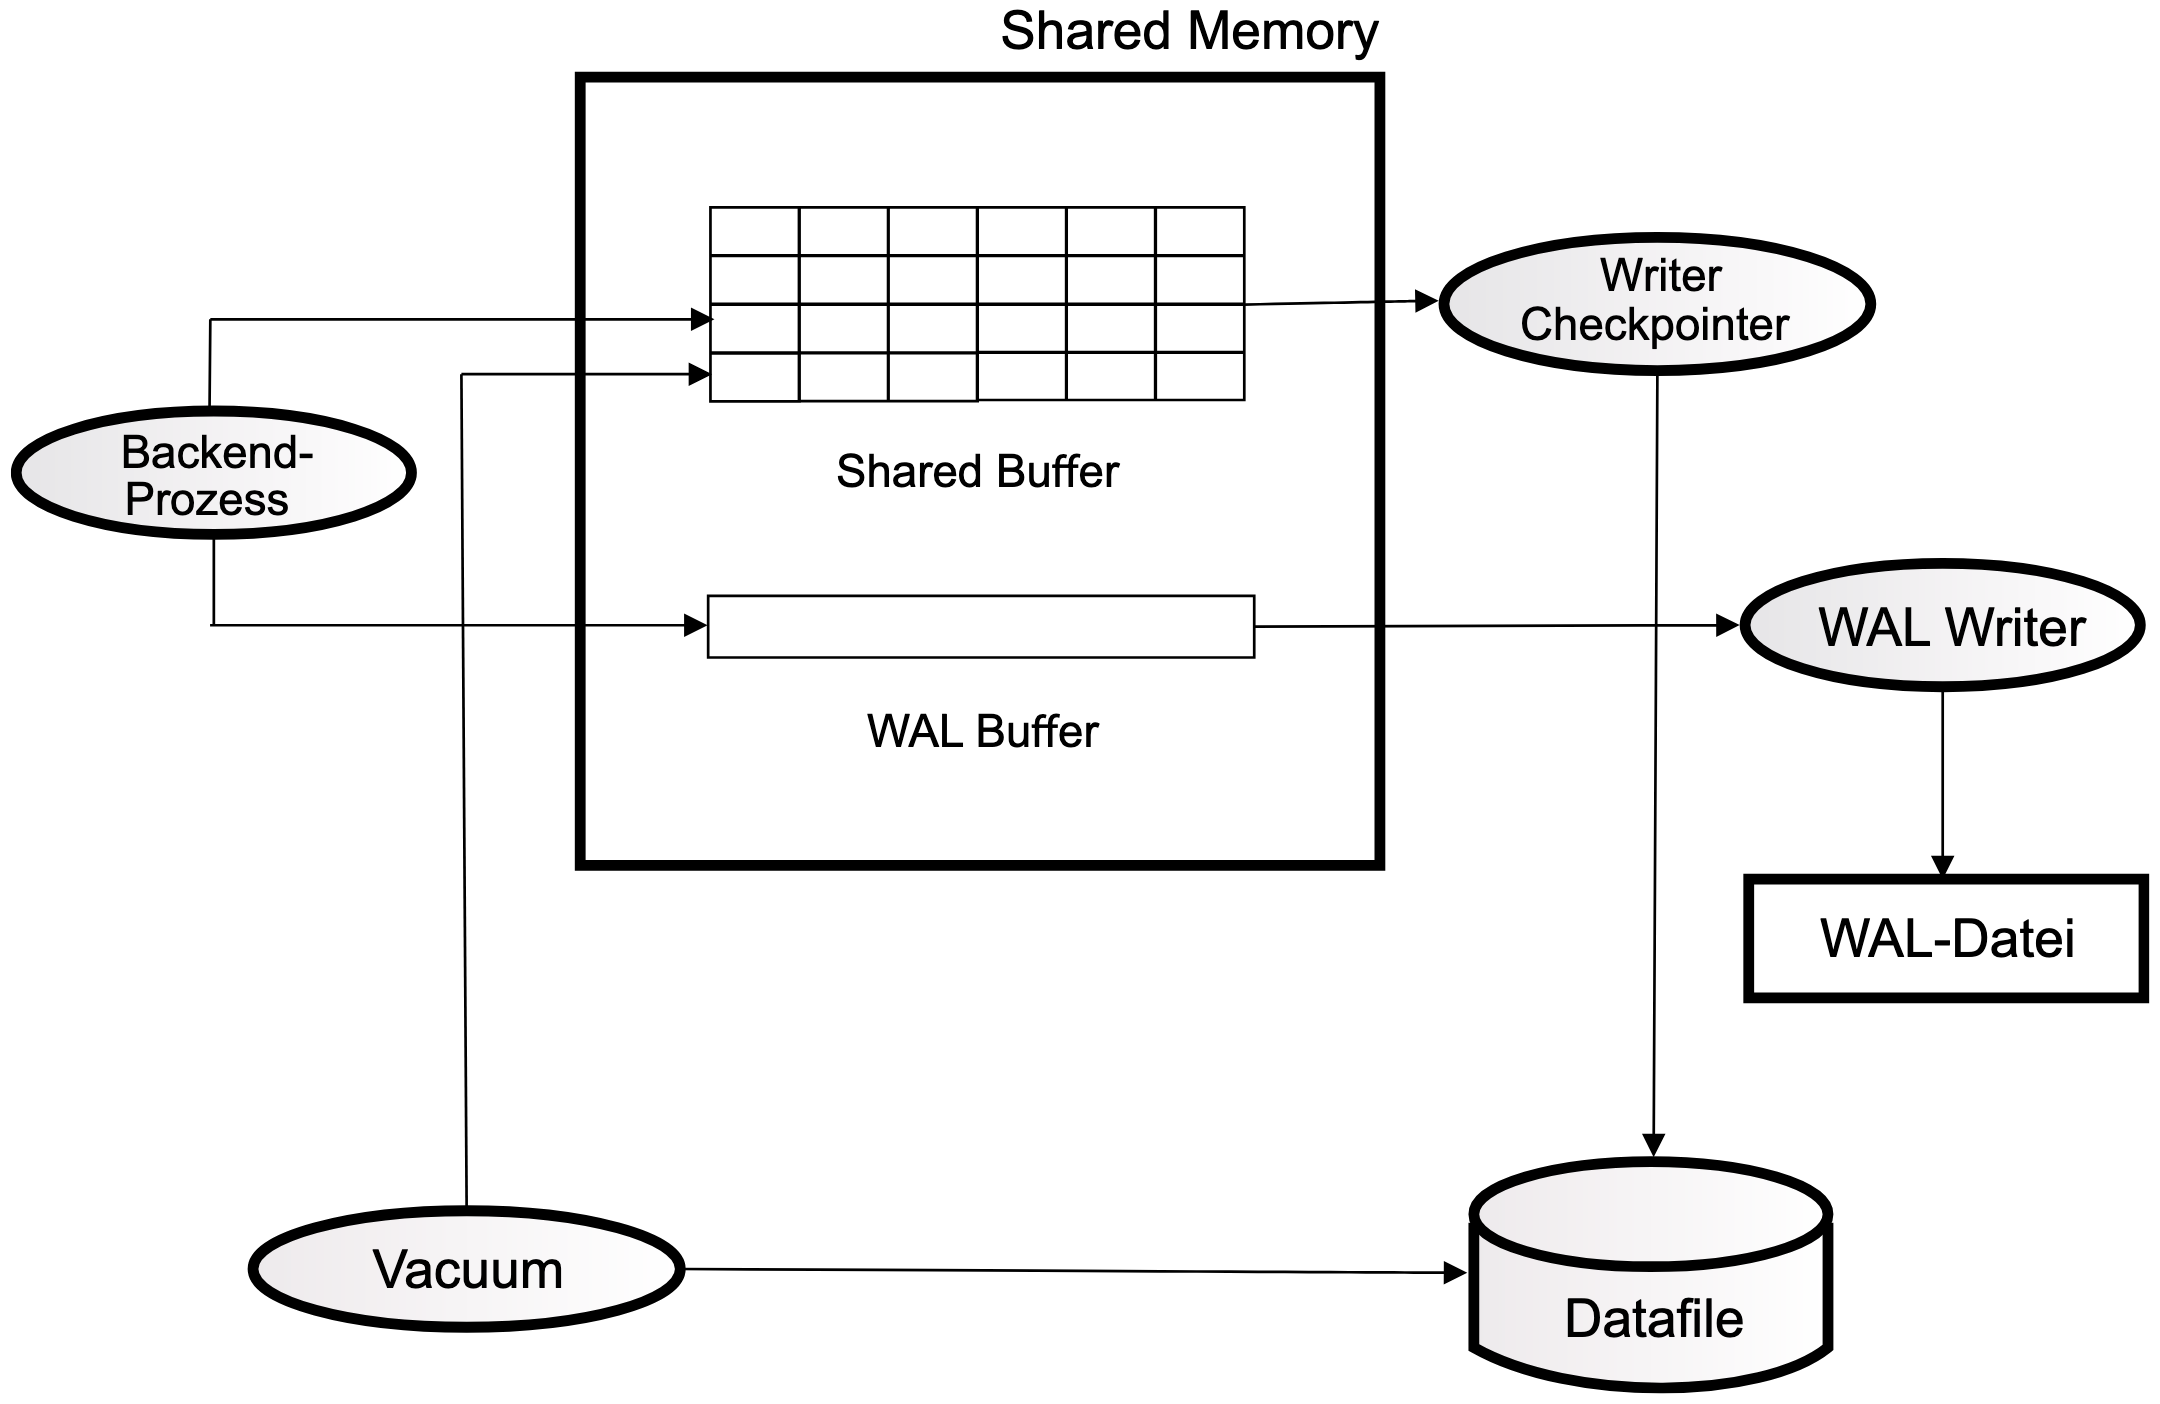
\includegraphics[width=\textwidth]{img/PostgreSQL Aufbau.png}
\caption{PostgreSQL Architektur. Quelle: \cite{Froehlich2022} S. 33 Bild 4.1}
\label{fig:Architektur}
\end{figure}

PostgreSQL besteht aus einer Kombination von Speicher und Prozessen. Bei Unix-Systemen sind diese Prozesse eigenständig, während sie bei Windows als Threads umgesetzt werden. Die wichtigsten Prozesse, die die Funktionalität von PostgreSQL abbilden, sind:
\begin{description}
    \item[Postmaster:] Der Hauptprozess, der die Verwaltung der anderen Prozesse übernimmt.
    \item[Checkpointer:] Dieser Prozess sorgt dafür, dass alle Änderungen in der Datenbank regelmäßig auf die Festplatte geschrieben werden.
    \item[Writer:] Verantwortlich für das Schreiben von geänderten Datenblöcken auf die Festplatte.
    \item[WAL Writer:] Handhabt das Schreiben von Transaktionsdaten in die Write-Ahead Log (WAL).
    \item[Autovacuum Launcher:] Dieser Prozess führt automatische Bereinigungen der Datenbank durch.
    \item[Archiver:] Archiviert die WAL-Dateien für eine verbesserte Rückverfolgbarkeit und Monitoring, besonders wichtig in produktiven Systemen.
    \item[Stats Collector:] Sammelt statistische Daten über die Nutzung von Sessions und Tabellen.
    \item[BGWorker:] Übernimmt verschiedene Hintergrundaufgaben.
\end{description}

\begin{figure}[h]
\centering
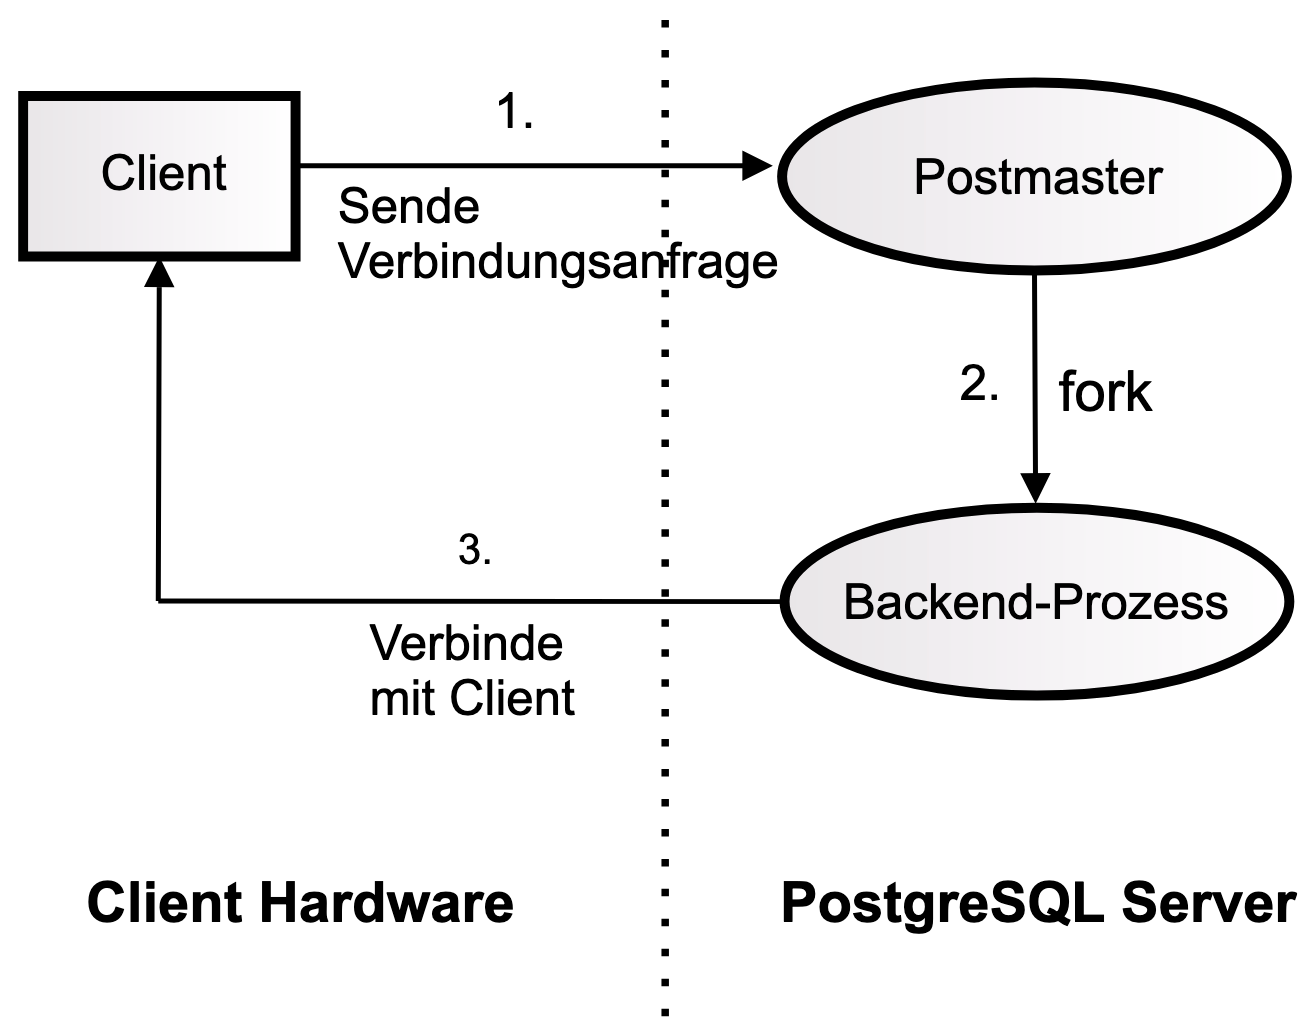
\includegraphics[width=\textwidth]{img/PostgreSQL Verbindungsaufbau.png}
\caption{Verbindungsaufbau von Client zum Server. Quelle: \cite{Froehlich2022} S. 35 Bild 4.3}
\label{fig:Verbindungsaufbau}
\end{figure}

Beim Aufbau einer Verbindung durch einen Client erstellt der Postmaster-Prozess nach erfolgreicher Authentifizierung und Autorisierung einen eigenen Backend-Thread. Die maximale Anzahl gleichzeitig aktiver Backend-Threads ist limitiert (Standard 100), was bedeutet, dass nach Erreichen dieser Grenze weitere Verbindungen abgelehnt werden.

\subsubsection{Speicherverwaltung und Performanceoptimierung}
Die Verwaltung von Speicher und die Optimierung der Zugriffszeiten auf Daten sind entscheidend für die Leistung von PostgreSQL. Da das Lesen von Daten von einer Festplatte vergleichsweise zeitaufwendig ist, setzt PostgreSQL auf verschiedene Mechanismen zur Verbesserung der Performance.

\begin{figure}[h]
\centering
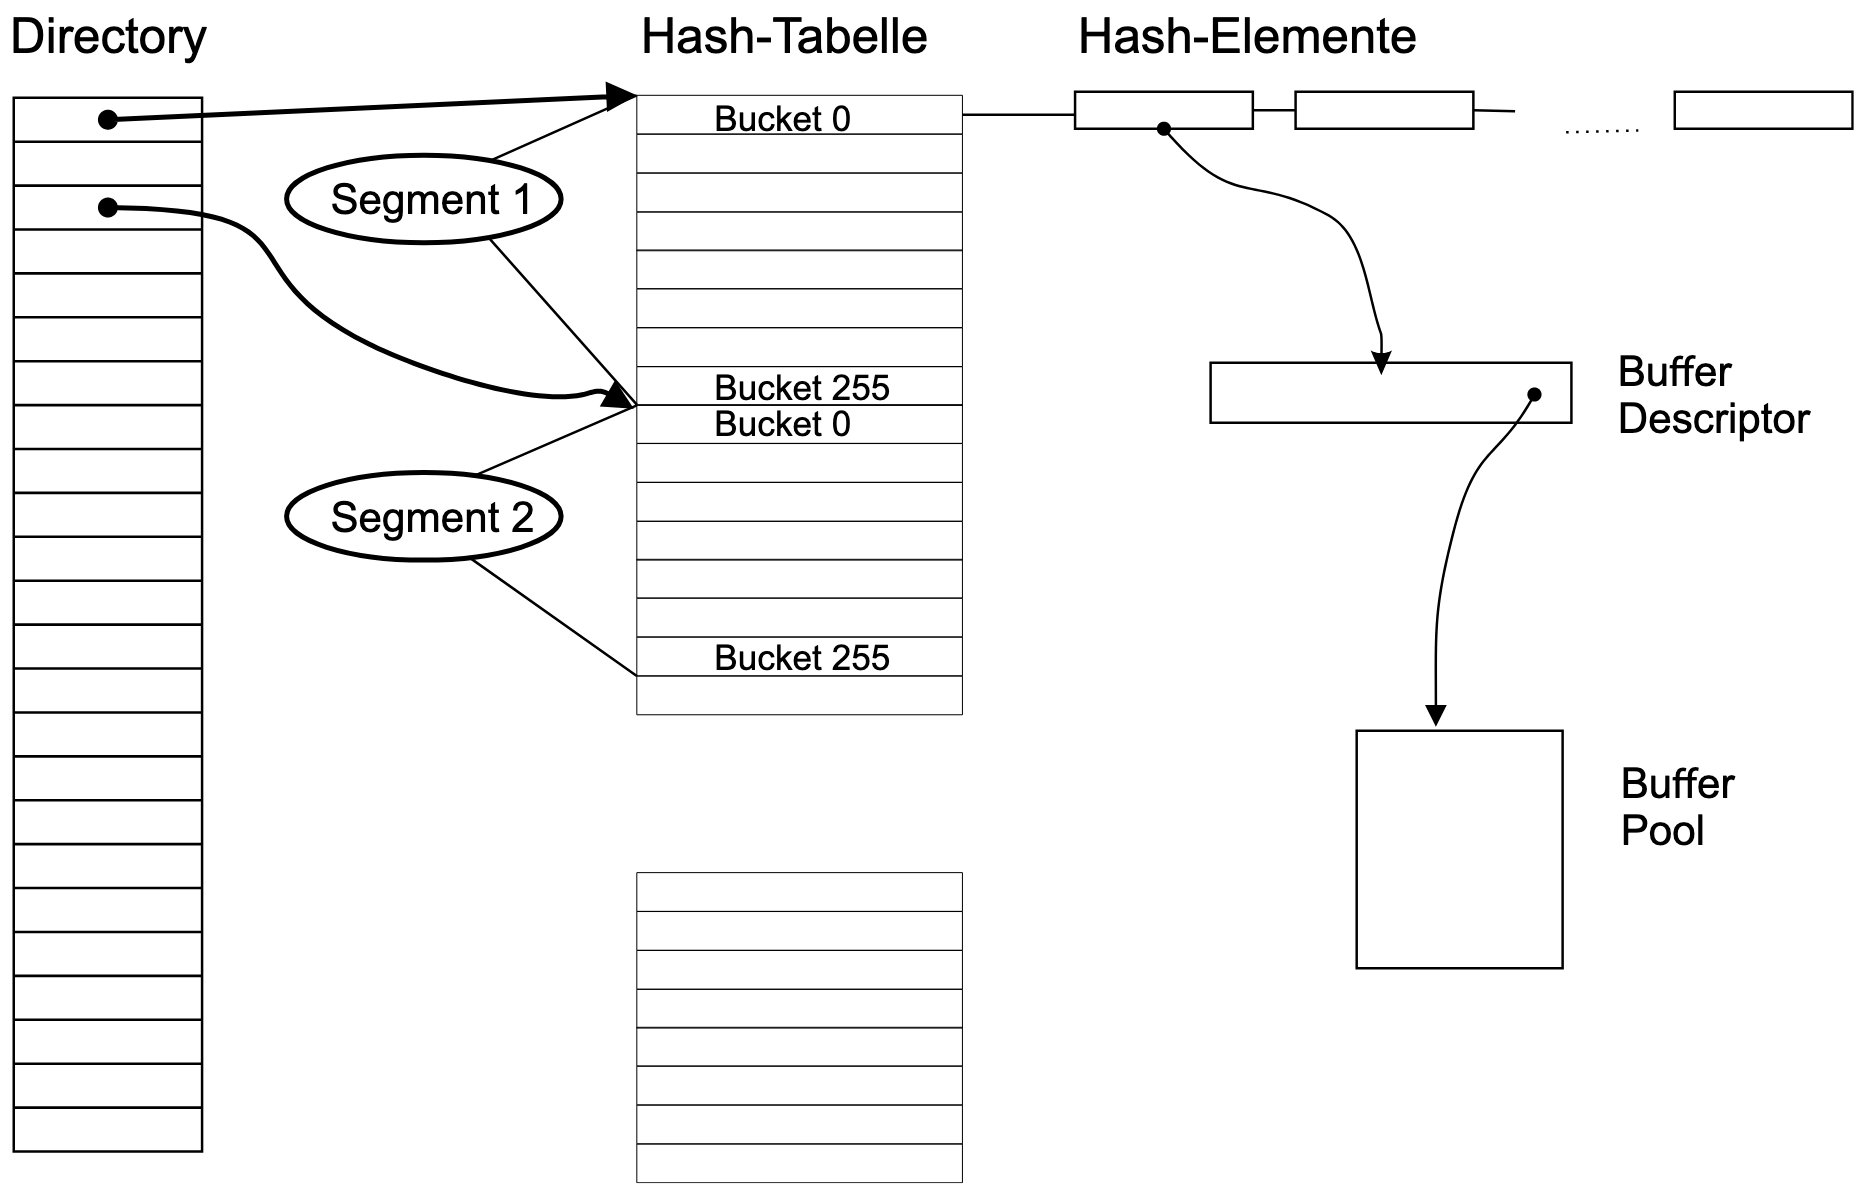
\includegraphics[width=\textwidth]{img/PostgreSQL Speciheraufbau.png}
\caption{PostgreSQL Speicherarchitektur. Quelle:  \cite{Froehlich2022} S. 37 Bild 4.4}
\label{fig:Speicheraufbau}
\end{figure}

\paragraph{Geteilter Speicher (Shared Buffer)}
Der Shared Buffer in PostgreSQL dient dazu, die Anzahl der Operationen auf der Festplatte zu reduzieren, indem er schnellen Speicher im RAM bereitstellt. Er besteht aus einer Hash-Tabelle, Hash-Elementen, einer Bufferbeschreibung und einer Buffersammlung. Die Hash-Tabelle ermöglicht ein schnelles Auffinden von Datensätzen, indem Hashwerte in Segmenten sortiert werden. Diese Segmente können sehr schnell durchsucht werden, da ihre Länge fest ist, was effiziente Speicherzugriffe ermöglicht.

Die Bufferbeschreibung enthält wichtige Steuerungsvariablen, wie z.B. den \code{\url{usage count}}, der die Relevanz eines Datensatzes im Speicher angibt. Der Speicherbereinigungsprozess (Eviction Process) durchsucht regelmäßig den Buffer nach irrelevanten Blöcken. Blöcke, die als irrelevant eingestuft werden, können überschrieben werden, sobald neuer Speicherplatz benötigt wird.

\paragraph{WAL Buffer und Checkpoints}
Der \ac{wal} Buffer ist darauf ausgelegt, Daten effizient auf die Festplatte zu schreiben. Dadurch müssen schreibende Prozesse nicht auf die tatsächliche Schreiboperation warten, sondern können die zu schreibenden Daten in den Buffer verlagern. Der \ac{wal} Buffer wird in regelmäßigen Intervallen (Standard 200 Millisekunden) überprüft und die Daten werden im Permanentspeicher gesichert, um die Ausfallsicherheit zu gewährleisten.

\code{Insert}-, \code{Update}- und \code{Delete}-Anweisungen werden über den \ac{wal}-Buffer verarbeitet. Diese Anweisungen werden in sogenannten \ac{wal}-Records gespeichert und sichern den Zustand der Daten auch bei einem Systemausfall. Ein Checkpoint, der den Speicherinhalt endgültig auf die Festplatte schreibt, wird unter bestimmten Bedingungen ausgeführt, wie etwa nach Ablauf eines festgelegten Intervalls, Erreichen einer bestimmten Buffergröße oder dem manuellen Auslösen eines Checkpoints.

\paragraph{Mehrere Datenblockversionen und Defragmentierung}

PostgreSQL unterstützt die gleichzeitige Bearbeitung von Datensätzen durch mehrere Sessions. Um sicherzustellen, dass sich die Sessions nicht gegenseitig beeinträchtigen, erhalten Datensätze eine Versionsnummer. Diese ermöglicht es, bei gleichzeitigen Abfragen und Bearbeitungen konsistente Daten bereitzustellen. Wenn eine Abfrage gestartet wird, kann anhand der Versionsnummer bestimmt werden, welcher Datensatz zum Zeitpunkt des Abfragestarts aktuell war.

Alte Datensätze, die nicht mehr benötigt werden, werden gelöscht, wodurch Lücken in der Tabelle entstehen. Diese Lücken werden durch den Autovacuum-Prozess freigegeben, sodass der Speicher für neue Datenblöcke verwendet werden kann. Bei Bedarf führt PostgreSQL ein \code{fullvacuum} durch, der die Tabelle vollständig defragmentiert, um Speicherplatz zurückzugewinnen und die Integrität der Versionsnummern zu gewährleisten.

\subsubsection{Permanentspeicherverwaltung}

Die Datenbanken von PostgreSQL werden im Verzeichnis \code{base} gespeichert, während der Tablespace in einem separaten Verzeichnis liegt. Tabellen und Indizes werden in Dateien von maximal einem Gigabyte Größe gespeichert; bei Überschreiten dieser Größe wird eine weitere Datei angelegt. Zusätzlich werden Dateien mit den Endungen \code{\_fsm} (Free Space Map) zur Adressierung des freien Speicherplatzes und \code{\_vm} (Visibility Map) zur Markierung von veralteten Datensätzen gepflegt.

Die Datenblocksammlung (Page) enthält Pointers auf die tatsächlichen Datenblöcke (Tuples). Jeder Datenblock wird durch eine Kombination aus der Datenblocksammlungsnummer und dem Offset des Pointers identifiziert. \cite{Froehlich2022}

\subsection{Exkurs: MongoDB}
MongoDB ist eine führende dokumentenorientierte NoSQL-Datenbank, die sich durch ihre Flexibilität und Skalierbarkeit auszeichnet. Sie wurde entwickelt, um einige der Einschränkungen traditioneller relationaler Datenbanken zu überwinden und bietet eine leistungsfähige Lösung für Anwendungen, die große Mengen an unstrukturierten oder semi-strukturierten Daten verarbeiten müssen. Im Gegensatz zu relationalen Datenbanken, die auf einem festen Schema basieren, erlaubt MongoDB ein dynamisches, schemaloses Datenmodell, das sich ideal für moderne, agile Entwicklungsprozesse eignet. In diesem Exkurs werden die Architektur und die technischen Merkmale von MongoDB detailliert beleuchtet, um deren Eignung für das \ac{nomtis}-Projekt zu bewerten.

\subsubsection{Speicherstruktur und Organisation}
MongoDB speichert Daten im \ac{bson}-Format, einem binären Format, das speziell für die Speicherung von Dokumenten mit \ac{json}-Syntax entwickelt wurde. \ac{bson} bietet eine effiziente Speicherung und Verarbeitung von Dokumenten, da es im Vergleich zu herkömmlichem \ac{json} kompakter und schneller zu verarbeiten ist. \ac{bson}-Dokumente können direkt in \ac{json} konvertiert werden, was die Integration mit Anwendungen erleichtert, die \ac{json} verwenden.

Die Speicherorganisation in MongoDB ist hierarchisch aufgebaut:
\begin{description}
    \item[Datenbank:] An der Spitze steht eine Datenbank, die mehrere Sammlungen (engl. Collections) enthalten kann.
    \item [Katalog:] Darunter befindet sich der Katalog, der Informationen über die Sammlungen und Indizes speichert.
    \item [Sammlung (engl. Collection)]: Eine Sammlung ist eine Gruppe von Dokumenten, die thematisch zusammengehören und ähnliche Strukturmerkmale aufweisen.
    \item [Dokument:] Auf der untersten Ebene steht das Dokument, das die eigentlichen Daten enthält.
\end{description}

\subsubsection{Katalog und Speicherverwaltung}

Der Katalog von MongoDB ist für die Verwaltung der Metadaten von Sammlungen und Indizes verantwortlich. Es gibt zwei Arten von Katalogen:
\begin{description}
    \item[Persistenter Katalog:] Dieser speichert Informationen dauerhaft auf der Festplatte und stellt sicher, dass Metadaten auch nach einem Neustart des Systems verfügbar bleiben. Der persistente Katalog wird in BSON-Dateien mit der Endung \code{\_mdb\_catalog} gespeichert und enthält Details über die Eigenschaften und Indizes der Sammlungen.
    \item [Memory-Katalog:] Der Memory-Katalog hält die Metadaten im RAM vor, um schnellen Zugriff zu gewährleisten und Ladezeiten zu minimieren. Operationen wie das Erstellen, Suchen, Iterieren und Schließen von Sammlungen werden im Memory-Katalog durchgeführt.
\end{description}

Um Dateninkonsistenzen zu vermeiden, wird der Memory-Katalog regelmäßig mit dem persistenten Katalog synchronisiert. Eine Versionsverwaltung stellt sicher, dass Änderungen korrekt nachvollzogen werden können, ohne dass es zu Lese-Schreib-Kollisionen kommt. MongoDB verwendet dabei das Copy-on-Write-Prinzip, bei dem nur dann eine Kopie des Datensatzes erstellt wird, wenn tatsächlich Änderungen vorgenommen werden. Dies minimiert den Speicherbedarf und erhöht die Effizienz.

\subsubsection{Speicherverwaltung und Defragmentierung}
Beim Löschen eines Eintrags in MongoDB erfolgt dieser Prozess in zwei Schritten:
\begin{enumerate}
    \item Löschen des Katalogeintrags: Zunächst wird der Eintrag sowohl im Memory-Katalog als auch im persistenten Katalog entfernt. Ein Verweis auf die Sammlung wird an den sogenannten \glqq Reaper\grqq{} übergeben, um sicherzustellen, dass keine neuen Zugriffe auf die Sammlung erfolgen, während aktive Lesezugriffe abgeschlossen werden.
    \item Endgültiges Löschen: Nachdem sichergestellt wurde, dass kein Rollback erfolgen kann, der die Daten der Sammlung wiederherstellen könnte, werden die Daten endgültig gelöscht.
\end{enumerate}

Freier Speicher, der durch das Löschen von Daten entsteht, wird in regelmäßigen Abständen für neue Datensätze freigegeben. Wenn der Speicher fragmentiert wird und viele kleine Lücken entstehen, führt MongoDB eine Defragmentierung durch. Dieser Prozess ordnet den Speicher neu an, kann jedoch Lese- und Schreiboperationen blockieren, was die Performance beeinträchtigen könnte. Daher sollte die Defragmentierung möglichst selten durchgeführt werden.

\subsubsection{Indizes und Abfragen}
Indizes in MongoDB werden hauptsächlich als B-Baum-Strukturen gespeichert, die eine effiziente Suche und Sortierung von Daten ermöglichen. Ein B-Baum-Index speichert die Daten strukturiert, ähnlich wie ein Dokument, und ermöglicht schnelle Zugriffe auf häufig abgefragte Felder. MongoDB erlaubt es auch, benutzerdefinierte Speicherstrukturen für Indizes zu erstellen, um spezifische Anwendungsanforderungen zu erfüllen. \cite{IamXander2024} \cite{themattman2024}

\subsubsection{BSON - Binary JSON}

\ac{bson} ist das zugrunde liegende Format für die Speicherung von Dokumenten in MongoDB. Es handelt sich dabei um ein binäres Format, das sogenannte Key-Value-Paare speichert und direkt in \ac{json} konvertiert werden kann. \ac{bson} ist jedoch deterministischer als \ac{json}, da es keine Flexibilität in der Darstellungsform bietet. Dies bedeutet, dass ein Datensatz in \ac{bson} immer in einer einzigen, festen Form dargestellt wird.

Ein \ac{bson}-Dokument beginnt immer mit einem 32-Bit-Ganzzahlwert, der die Länge des Dokuments angibt, und endet mit einem Null-Byte. Aufgrund dieser Struktur kann ein \ac{bson}-Dokument maximal ca. 2,147 Gigabyte an Daten umfassen. Die verschiedenen Datentypen, die \ac{bson} unterstützt, umfassen unter anderem:
\begin{description}
    \item[Int32 und Int64:] 4- bzw. 8-Byte lange Ganzzahlen.
    \item[Double:] 8-Byte lange Gleitkommazahlen nach dem IEEE 754-Standard.
    \item[Decimal128:] 16-Byte lange Gleitkommazahlen für hohe Präzision.
    \item[Array:] Ein Feld, das eine Liste von Werten speichert, wobei die Elemente wie Dokumente behandelt werden.
    \item[Null-Wert:] Ein spezieller Marker, der das Fehlen eines Wertes kennzeichnet.
    \item[Min- und Max-Schlüssel:] Marker, die den minimalen bzw. maximalen Wert eines Feldes darstellen.
\end{description}

Die strikte Struktur von \ac{bson} sorgt für eine konsistente und effiziente Speicherung und Verarbeitung von Dokumenten, was MongoDB zu einer leistungsfähigen Lösung für Anwendungen macht, die flexible und skalierbare Datenbanken benötigen. \cite{Velikhov}

\subsection{Diskurs: Vergleich von PostgreSQL und MongoDB für NOMTIS}
Die Auswahl der geeigneten Datenbanklösung ist ein zentraler Aspekt bei der Entwicklung von \ac{nomtis}. Da die internen Richtlinien PostgreSQL und MongoDB als verfügbare Optionen vorsehen, ist es entscheidend, die spezifischen Anforderungen von \ac{nomtis} zu analysieren und zu bestimmen, welche der beiden Datenbanken diese am besten erfüllt.

\subsubsection{Technische Anforderungen an NOMTIS}
\ac{nomtis} muss Benachrichtigungen effizient speichern, verwalten und flexibel verarbeiten können. Ein Hauptmerkmal von \ac{nomtis} ist die Fähigkeit, Benachrichtigungen mit potenziell komplexen und verschachtelten Datenstrukturen zu verwalten. Diese Datenstrukturen können variieren und sind oft nicht im Voraus vollständig definiert. Zudem sind eine hohe Zuverlässigkeit, Konsistenz und Skalierbarkeit erforderlich, um den Anforderungen eines modernen Benachrichtigungssystems gerecht zu werden.

\subsubsection{PostgreSQL: Technische Stärken und Grenzen}
PostgreSQL ist eine relationale Datenbank, die für ihre starke Unterstützung von \ac{acid}-Transaktionen, Datenintegrität und komplexen relationalen Abfragen bekannt ist. Diese Eigenschaften machen PostgreSQL ideal für Anwendungen, bei denen strenge Konsistenzanforderungen und komplexe Datenbeziehungen im Vordergrund stehen.

Die feste Struktur von PostgreSQL kann jedoch zu Einschränkungen führen, wenn es darum geht, dynamische und verschachtelte Datenstrukturen zu verwalten. Änderungen am Datenmodell erfordern eine Anpassung des Schemas, was in einem dynamischen Umfeld, wie es \ac{nomtis} erfordert, potenziell problematisch sein kann. Zudem ist PostgreSQL weniger effizient im Umgang mit tief verschachtelten oder unvorhersehbaren Datenstrukturen, was die Flexibilität des Systems einschränken könnte.

\subsubsection{MongoDB: Flexibilität und Skalierbarkeit}
MongoDB hingegen ist eine dokumentenorientierte NoSQL-Datenbank, die sich durch ihre schemalose Architektur und hohe Flexibilität auszeichnet. Die Speicherung erfolgt im BSON-Format, das eine effiziente Handhabung von \ac{json}-ähnlichen Dokumenten ermöglicht. Diese Struktur erlaubt es, Daten ohne festes Schema zu speichern, was für \ac{nomtis} von Vorteil ist, da die Benachrichtigungen beliebig komplexe und verschachtelte Daten enthalten können.

Ein weiterer zentraler Vorteil von MongoDB ist seine horizontale Skalierbarkeit. MongoDB unterstützt das sogenannte \glqq Sharding \grqq, bei dem Daten über mehrere Server verteilt werden, um eine hohe Verfügbarkeit und Performance sicherzustellen. Diese Fähigkeit zur horizontalen Skalierung ist besonders in einer Umgebung wie der \ac{sit} von Bedeutung, wo das Datenvolumen und die Anzahl der Nutzer kontinuierlich wachsen können.

Laut einer Untersuchung der MongoDB-Datenbank von Anjali Chauhan bietet MongoDB darüber hinaus eine hohe Leistung durch die Verwendung eingebetteter Datenmodelle, die E/A-Aktivitäten reduzieren, sowie durch Indizes, die schnellere Abfragen ermöglichen. \cite{Chauhan2019}
Diese Leistungsmerkmale machen MongoDB besonders geeignet für Anwendungen, die auf hohe Geschwindigkeit und effizienten Datenzugriff angewiesen sind.

\subsubsection{Schlussfolgerung: PostgreSQL als geeignete Wahl für Sensora}
Im Projekt Sensora ergibt sich aus den strukturellen Anforderungen und den funktionalen Zugriffsmustern ein klarer Bedarf an einem relationalen, transaktional konsistenten Datenbanksystem. Die Datenstruktur ist vordefiniert und weitgehend stabil. Pflanzen, Sensoren, Aktoren, Gruppen und Räume bilden klar abgegrenzte Entitäten mit definierten Beziehungen zueinander. Diese Relationen sind nicht nur logisch konzipiert, sondern stellen funktionale Notwendigkeiten dar – etwa wenn Sensoren bestimmten Pflanzen zugeordnet sind oder Aktionen nur innerhalb definierter Gruppenzugehörigkeiten zulässig sind.

Die Abfrageanforderungen im operativen Betrieb bestehen aus einer Mischung aus punktuellen Zugriffen (etwa auf aktuelle Sensorwerte oder Soll-Ist-Vergleiche) und zeitbasierten Auswertungen über große Datenmengen – insbesondere für die letzten 24 Stunden. Diese Anforderungen sind auf ein konsistentes, indexoptimiertes Schema angewiesen, das Joins effizient unterstützt und sich nicht durch Schema-Flexibilität, sondern durch strukturelle Integrität auszeichnet. Gleichzeitig ist paralleler Zugriff durch mehrere Microservices erforderlich, sodass Transaktionssicherheit und Isolation nicht nur erwünscht, sondern notwendig sind, um Inkonsistenzen bei konkurrierenden Schreiboperationen zu vermeiden.

PostgreSQL bietet genau für diese Art von Workload die passende Grundlage. Die stark normierten Strukturen des Sensora-Datenmodells profitieren von PostgreSQLs ausgefeilter Optimierung relationaler Abfragen, der zuverlässigen Durchsetzung referenzieller Integrität sowie der Möglichkeit, durch gezieltes Indexing auf Zeitstempel-Feldern hochfrequente historische Abfragen performant abzubilden. Selbst bei wachsendem Datenvolumen lassen sich durch Partitionierung oder die spätere Ergänzung durch TimescaleDB – ohne Verlassen der PostgreSQL-Basis – die Performanceanforderungen langfristig erfüllen, ohne strukturelle Kompromisse einzugehen.

Die fehlende Notwendigkeit für dynamische Schemas, polymorphe Dokumente oder eingebettete Strukturen eliminiert die Hauptargumente für ein dokumentenbasiertes System wie MongoDB. Vielmehr würde dessen Flexibilität in diesem Kontext eher potenzielle Inkonsistenzen begünstigen und zusätzliche Validierungslogik auf Anwendungsebene erforderlich machen – ein Mehraufwand, der durch das klar strukturierte Datenmodell nicht gerechtfertigt ist.

In Summe ist PostgreSQL damit nicht nur die technisch bessere Wahl, sondern die natürlichere Fortsetzung der bereits im Projektdesign angelegten Prinzipien: strukturierte, konsistente und integrierte Datenhaltung, auf die performant und sicher gleichzeitig von vielen Systemkomponenten zugegriffen werden kann.

	%%Auswahl der Technologien für eine Kompüonente des Projektes, basierend auf den Anforderungen, die in der vorherigen Sektion definiert wurden (Zentral für die Arbeit)
\section{IoT Device}
Das IoT Device ist ein zentraler Bestandteil des Projektes. Es ist dafür verantwortlich, die Daten von den Sensoren zu sammeln und an die Cloud zu übertragen. In diesem Abschnitt werden die Technologien ausgewählt, die für das IoT Device verwendet werden sollen. Die Auswahl erfolgt auf Basis der Anforderungen, die in der vorherigen Sektion definiert wurden.
\subsection{Verfügbare Technologien}
Die folgenden Technologien sind verfügbar.
\subsection{State of the Art Technologie}
Die Technologie 1 ist State of the Art und wird oft für IoT Devices verwendet.
\subsection{Vergleich von Technologien}
Die Technologien erfüllen die Anforderungen wie folgt:
\begin{itemize}
    \item Technologie 1: erfüllt die Anforderungen A, B und C.
    \item Technologie 2: erfüllt die Anforderungen A, B und D.
    \item Technologie 3: erfüllt die Anforderungen A, C und D.
\end{itemize}
\subsection{Auswahl der Technologie}
Die Technologie 1 wird ausgewählt, da sie die Anforderungen A, B und C erfüllt. Die Technologie 2 wird nicht ausgewählt, da sie die Anforderungen A, B und D erfüllt, aber nicht so gut wie Technologie 1. Die Technologie 3 wird ebenfalls nicht ausgewählt, da sie die Anforderungen A, C und D erfüllt, aber nicht so gut wie Technologie 1.
%Alternativ: Die technologie wird trotz ihre Status als State of the Art nicht ausgewählt, da sie die Anforderungen nicht ausreichend erfüllt.
	\newpage
	\chapter{Umsetzung}
	\section{Beschreibung des Datenbankaufbaus}
Die Datenbank des Systems Sensora ist im Schema sensora organisiert und verfolgt eine klar strukturierte, relationale Modellierung mit durchdachter Referentialität und Typisierung. Sie unterstützt die zentralen Funktionen des Systems wie Benutzerverwaltung, Gruppenzugehörigkeit, Raum- und Pflanzenzuordnung sowie Sensor- und Steuerdaten.
\newpage
\begin{figure}[H]
\centering
%  \includesvg[width=\linewidth, height=0.9\textheight, keepaspectratio,inkscapelatex=false]{img/Datenbank Diagramm.svg}
  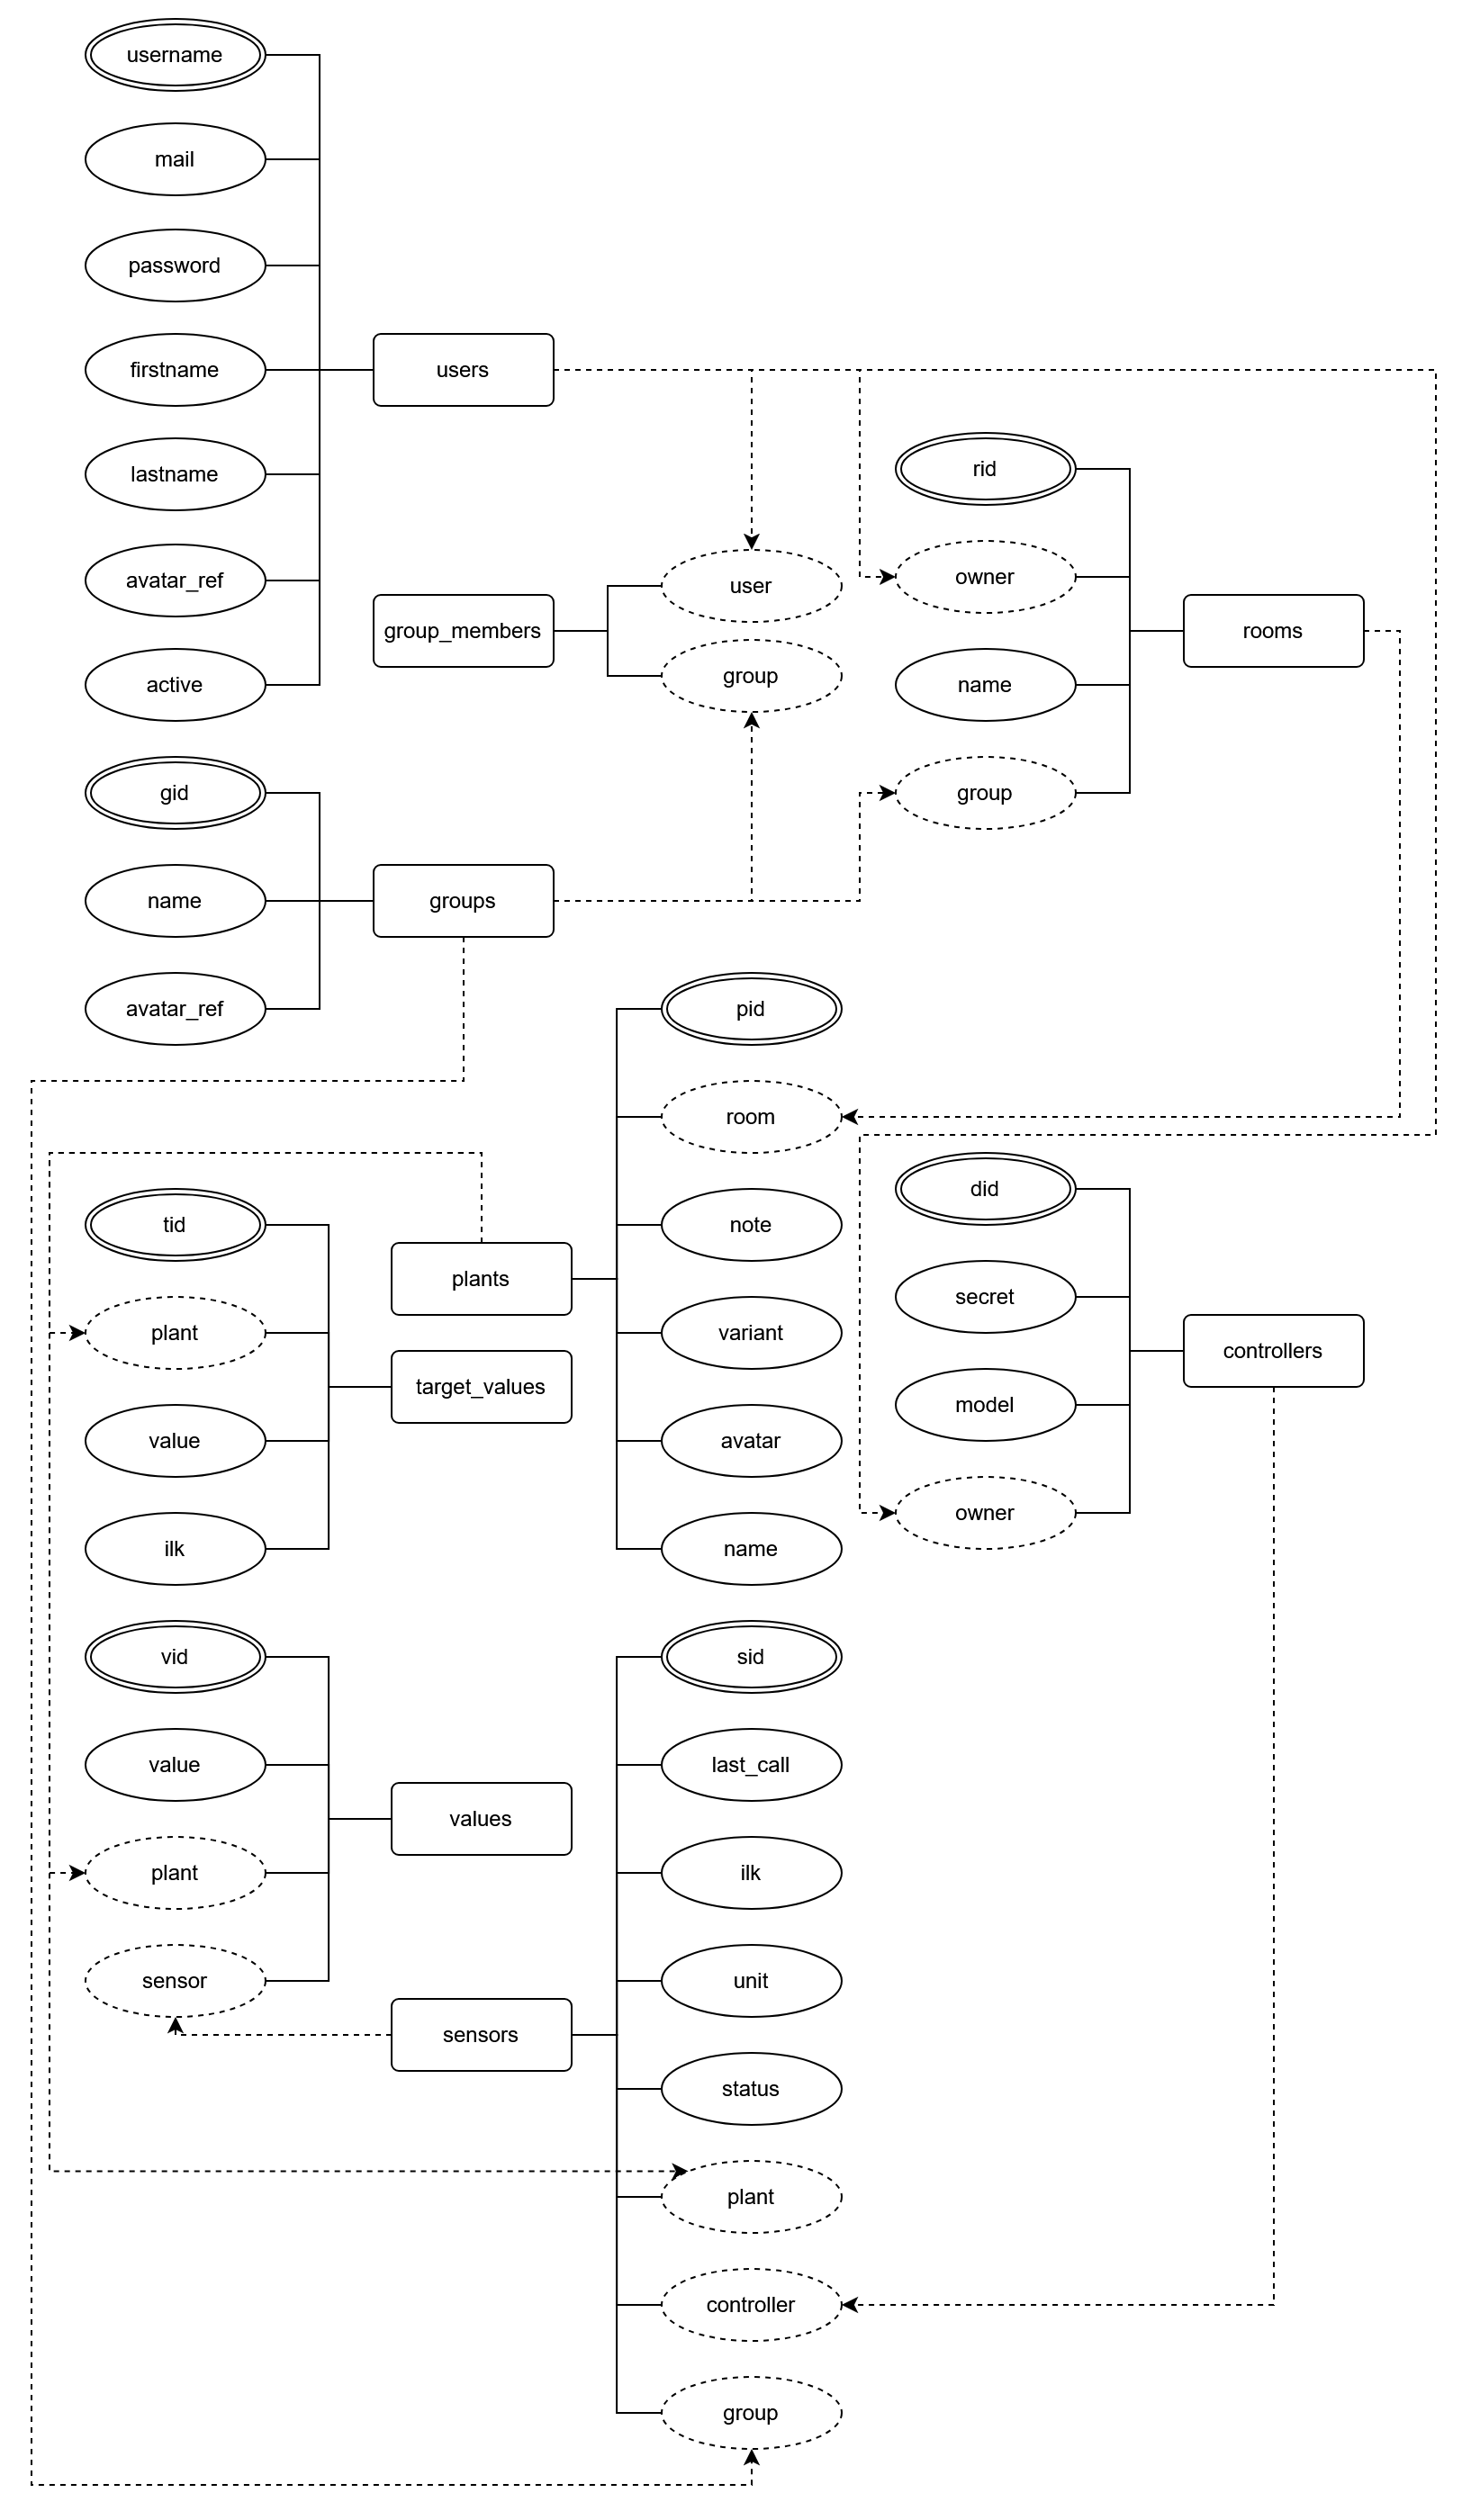
\includegraphics[width=\linewidth, height=0.9\textheight]{img/Datenbank Diagramm.png}
\caption{Sensora Datenbank Struktur}
\label{fig:sensora_datenbank}
\end{figure}
\newpage

\subsection{Struktur und Besonderheiten}
\begin{description}
    \item[Benutzerverwaltung:]
    Die Tabelle users bildet die zentrale Entität für Benutzer ab. Jeder Benutzer besitzt Pflichtangaben sowie einen referenzierten Avatar aus dem dedizierten ENUM-Typ sensora.avatar. Die E-Mail-Adresse ist eindeutig.
    \item[Gruppen \& Mitgliedschaften:]
    Gruppen (groups) können mehrere Mitglieder haben, realisiert durch die Join-Tabelle group\_members. Diese bildet eine klassische Many-to-Many-Beziehung zwischen Nutzern und Gruppen ab.
    \item[Räume \& Pflanzen:]
    Räume (rooms) können Gruppen zugeordnet sein und besitzen jeweils einen Eigentümer. Pflanzen (plants) sind immer einem Raum zugeordnet und dienen als Ankerpunkt für Messwerte.
    \item [Sensorik \& Steuerung:]
    Sensoren (sensors) sind mit Controllern (controllers) verknüpft und optional direkt mit einer Pflanze oder Gruppe verbunden. Jeder Sensor verwendet den ENUM-Typ sensora.status, um seinen Zustand zu klassifizieren.
    \item [Zielwerte \& Messdaten:]
    Pflanzen können über target\_values Zielgrößen definieren. Tatsächliche Messwerte werden in der Tabelle values gespeichert und jeweils einem Sensor sowie einer Pflanze zugeordnet.
\end{description}

\subsection{Technische Merkmale}
\begin{itemize}
    \item Es kommen ENUM-Typen zum Einsatz, um Felder wie Avatar und Status typensicher und standardisiert zu definieren.
    \item Sämtliche Fremdschlüsselbeziehungen nutzen CASCADE-Strategien zur Pflege von Konsistenz (z.B. beim Löschen von Benutzern oder Pflanzen).
    \item Indizes auf eindeutige Felder (z.B. mail, secret) erhöhen die Performanz gezielter Abfragen.
    \item Die Nutzung von Timestamps mit Standardwerten erlaubt eine automatische Protokollierung von Ereignissen wie Sensoraktivität.
\end{itemize}

Diese Datenbankstruktur ermöglicht eine flexible, erweiterbare und gleichzeitig robuste Grundlage für die Backend-Logik und garantiert eine nachvollziehbare Abbildung der fachlichen Entitäten.
	%%Hier wird alles beschrieben und erklärt, was während in der Praxis passiert ist und gemacht wurde.
\section{Umsetzung des IoT Devices}
Das IoT Device wurde von einer Person als Hauptentwickler und mehreren Unterstützenden Entwicklern erstellt.
    \subsection{Hardware}:
    Für die Hardware wurde ein fertiger Bausatz von Alibaba gekauft, der alle benötigten Komponenten enthielt.
    Darunter ein ESP32, sensoren und eine Pumpe.
    Die Hardware wurde zusammengebaut und testweise in Betrieb genommen, yada yada yada.
    \subsection{Software}:
    Die SOftware wurde in C Entwickelt.
    Es wurden die Komponenten x, y und z implementiert.
    Dabei lief dies gut und das nicht so gut.
   
	\newpage
	
	% ------------- Ende Hautpteil -------------
	
	\chapter{Kritische Reflexion}
	%%Reflektiere über umsetzung der Komponenten, was hat gut funktioniert, was nicht, was war einfach, was war schwer, was war unerwartet, was war nicht so gut.
\section{IoT Device}
Das IoT Device wurde von einer Person als Hauptentwickler und mehreren Unterstützenden Entwicklern erstellt.
    \subsection{Hardware}:
    Geplant war das IoT Device als ein Gerät, das die Luftfeuchtigkeit und Temperatur misst und diese Daten an einen Server sendet.
    Für die Hardware wurde ein fertiger Bausatz von Alibaba gekauft, der alle benötigten Komponenten enthielt. Damit war es möglich, die Hardware schnell zusammenzubauen und zu testen.
    Die Sensoren sind nur mittelmäßig genau, was aber für ein Proof of Concept ausreichend ist.
    \subsection{Software}:
    Die Software wurde in C entwickelt. Dabei wurde CLion mit CMake als IDE verwendet.
    Dadurch kam es zu komplikationen im Setup, da die IDE nicht richtig konfiguriert war. Daraus resultierten verzögerungen die das Projekt belasteten
    Mehr feste Entwickler hätten hier helfen können.

Insgesamt lief die Entwicklung des IoT Devices gut, aber es gab einige Herausforderungen, die bewältigt werden mussten.
    Die Hardware war einfach zusammenzubauen, aber die Software war schwieriger zu implementieren als erwartet.
    Es gab einige Probleme mit der Kommunikation zwischen dem IoT Device und dem Server, die behoben werden mussten.
    Auch die Genauigkeit der Sensoren war nicht so hoch wie erhofft, was die Ergebnisse beeinflusste.
    Dennoch konnte das IoT Device erfolgreich entwickelt und getestet werden, und es erfüllt die Anforderungen des Projekts.
    
	\newpage 
	\chapter{Ausblick}
	%% Hier bisschen Tagträumen was in Zukunft noch so kommen könnte.
\section{IoT Device}
Das IoT Device könnte in Zukunft durch bessere Sensoren und eine bessere Software weiter verbessert werden.
Mehr Modularität könnte auch helfen, das IoT Device einfacher zu erweitern und anzupassen.
Das IoT Device könnte auch in Zukunft durch eine bessere Benutzeroberfläche und eine bessere Integration in andere Systeme weiter verbessert werden.
	\newpage
	
	%------------- Literaturverzeichnis -------------
	\newpage
	\pagestyle{fancy}
	\fancyhead[R]{LITERATUR}

	\chapter*{Literaturverzeichnis}
	\addcontentsline{toc}{chapter}{Literaturverzeichnis}
	\printbibliography
	\newpage

	%------------- Anhang -------------
	\cleardoublepage
	\fancyhead[R]{ANHANG}

	\chapter*{Anhang}
	\addcontentsline{toc}{chapter}{Anhang}

	% Hier Anhänge einfügen:
	%\input{./Anhang/sensorwerte}
	%\input{./Anhang/schaltplan}

\newpage

	
\end{document}